\begin{frame}{Roteiro}
    \textbf{Objetivo:} Limitar a largura arbórea de grafos $k$-outerplanar.\\
    \pause\bigbreak
    \textbf{Plano:}\\
    \vspace{0.2cm}
    \hspace{0.4cm}\textbf{Passo 1}: Considerar apenas grafos $k$-outerplanar de grau máximo $3$\\
    \pause
    \vspace{0.1cm}
    \hspace{0.4cm}\textbf{Passo 2}: Provar que grafos $k$-outerplanar de grau máximo três têm carga máxima limitada\\
    \pause
    \vspace{0.1cm}
    \hspace{0.4cm}\textbf{Passo 3}: Provar que carga máxima limitada implica em largura arbórea limitada
\end{frame}

\begin{frame}{Passo 1}
    \begin{lema}
        Todo grafo $k$-outerplanar $G$ pode ser transformado em um grafo $k$-outerplanar $G^{\prime}$ de grau máximo 3, tal que uma decomposição em árvore de $G^{\prime}$ corresponde a uma de $G$ de mesma largura.
    \end{lema}
    \begin{proof}
        Divida qualquer vértice $v$ de grau $d$ maior que $3$ em dois vértices $v_1, v_2$ de grau $3$ e $d-1$.\\
        \vspace{0.2cm}
        \begin{minipage}{\linewidth}
            \centering
            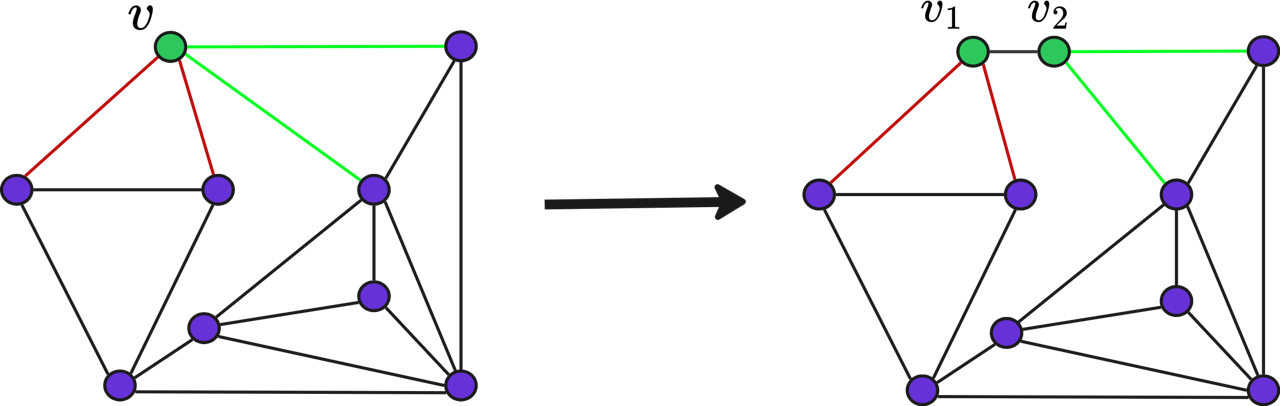
\includegraphics[width=6cm]{images/proof_1_1.png}
        \end{minipage}\\
        \vspace{0.4cm}
        Se $v_{1}$ ou $v_{2}$ estão em $X^{\prime}_{i}$, definimos $X_{i}=\{X^{\prime}_{i}\setminus\{v_{1}, v_{2}\}\} \cup \{v\}$; senão $X_{i}=X^{\prime}_{i}$. \phantom{\qedhere}
    \end{proof}
\end{frame}

\begin{frame}{Passo 1\dots}
    \begin{proof}
        \begin{itemize}[-]
            \item Crie uma sequência de decomposições $G_{1}, G_{2}, \dots, G_{z}$ tal que $G_{z}$ tem grau máximo $3$;
            \item Obtenha uma decomposição em árvore de $G_z$;
            \item Construa decomposições para $G_{z-1}, G_{z-2}, \dots, G_1, G$, de tal forma que a decomposição final de $G$ tenha largura no máximo igual à de $G_z$.
        \end{itemize}
        \alt<4>{\qedhere}{\phantom\qedhere}
    \end{proof}
\end{frame}

\begin{frame}{Definições Que Nunca Acabam}
    \Large{Dada uma floresta geradora maximal $(V, F)$ de um grafo $G$, e uma aresta $e \in E \setminus F$:}
    \bigbreak

    \begin{defi}[Ciclo fundamental]
        O \emph{\textbf{ciclo fundamental}} de $e$ é o ciclo formado ao adicionar $e$ à $F$.
    \end{defi}
\end{frame}

\begin{frame}{Definições Que Nunca Acabam}
    \begin{defi}[Carga de vértice]
        A \emph{\textbf{carga de um vértice}} $v \in V$ é o número de ciclos fundamentais em que $v$ aparece.
    \end{defi}

    \begin{defi}[Carga aresta]
        A \emph{\textbf{carga de uma aresta}} $e \in F$ é o número de ciclos fundamentais que a contêm.
    \end{defi}
\end{frame}

\begin{frame}{Quiz}
    \centering\Large
    Encontre a carga do vértice e aresta vermelhos\bigbreak
    \begin{minipage}{\linewidth}
        \centering
        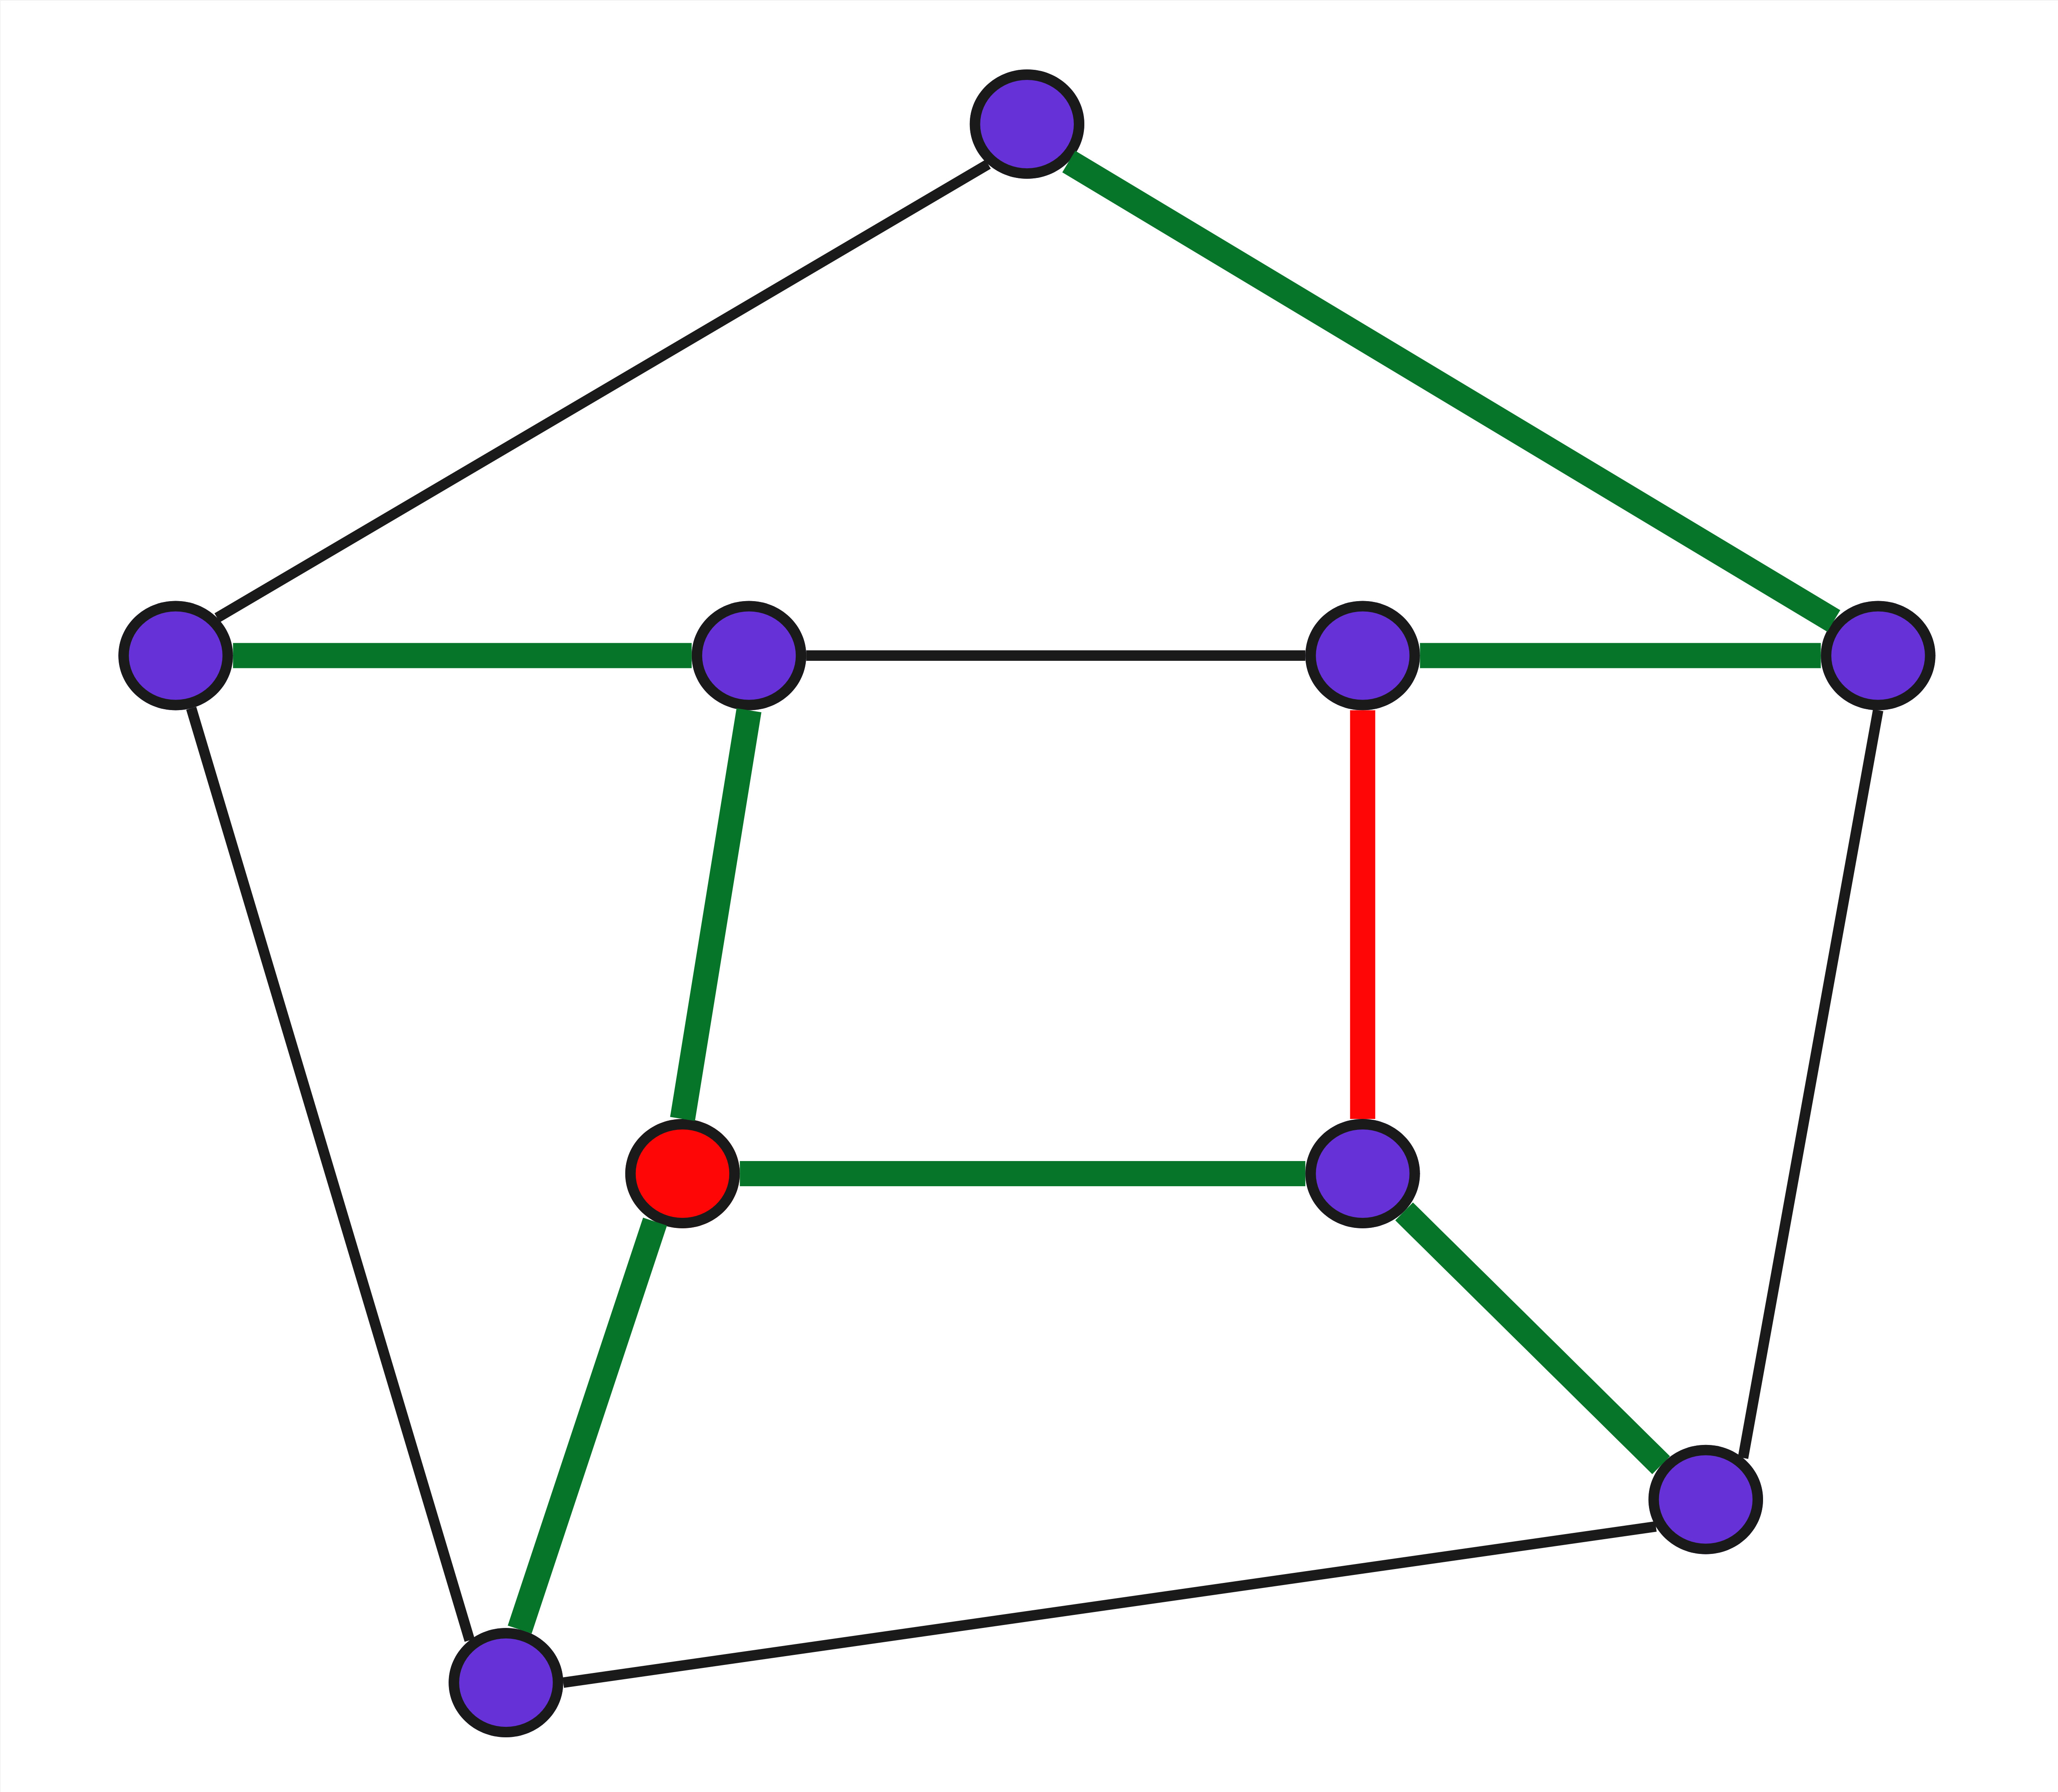
\includegraphics[width=7cm]{images/load_1.jpg}
    \end{minipage}
\end{frame}

\begin{frame}{Quiz}
    \centering\Large
    Encontre a carga do vértice e aresta vermelhos\bigbreak
    \begin{minipage}{\linewidth}
        \centering
        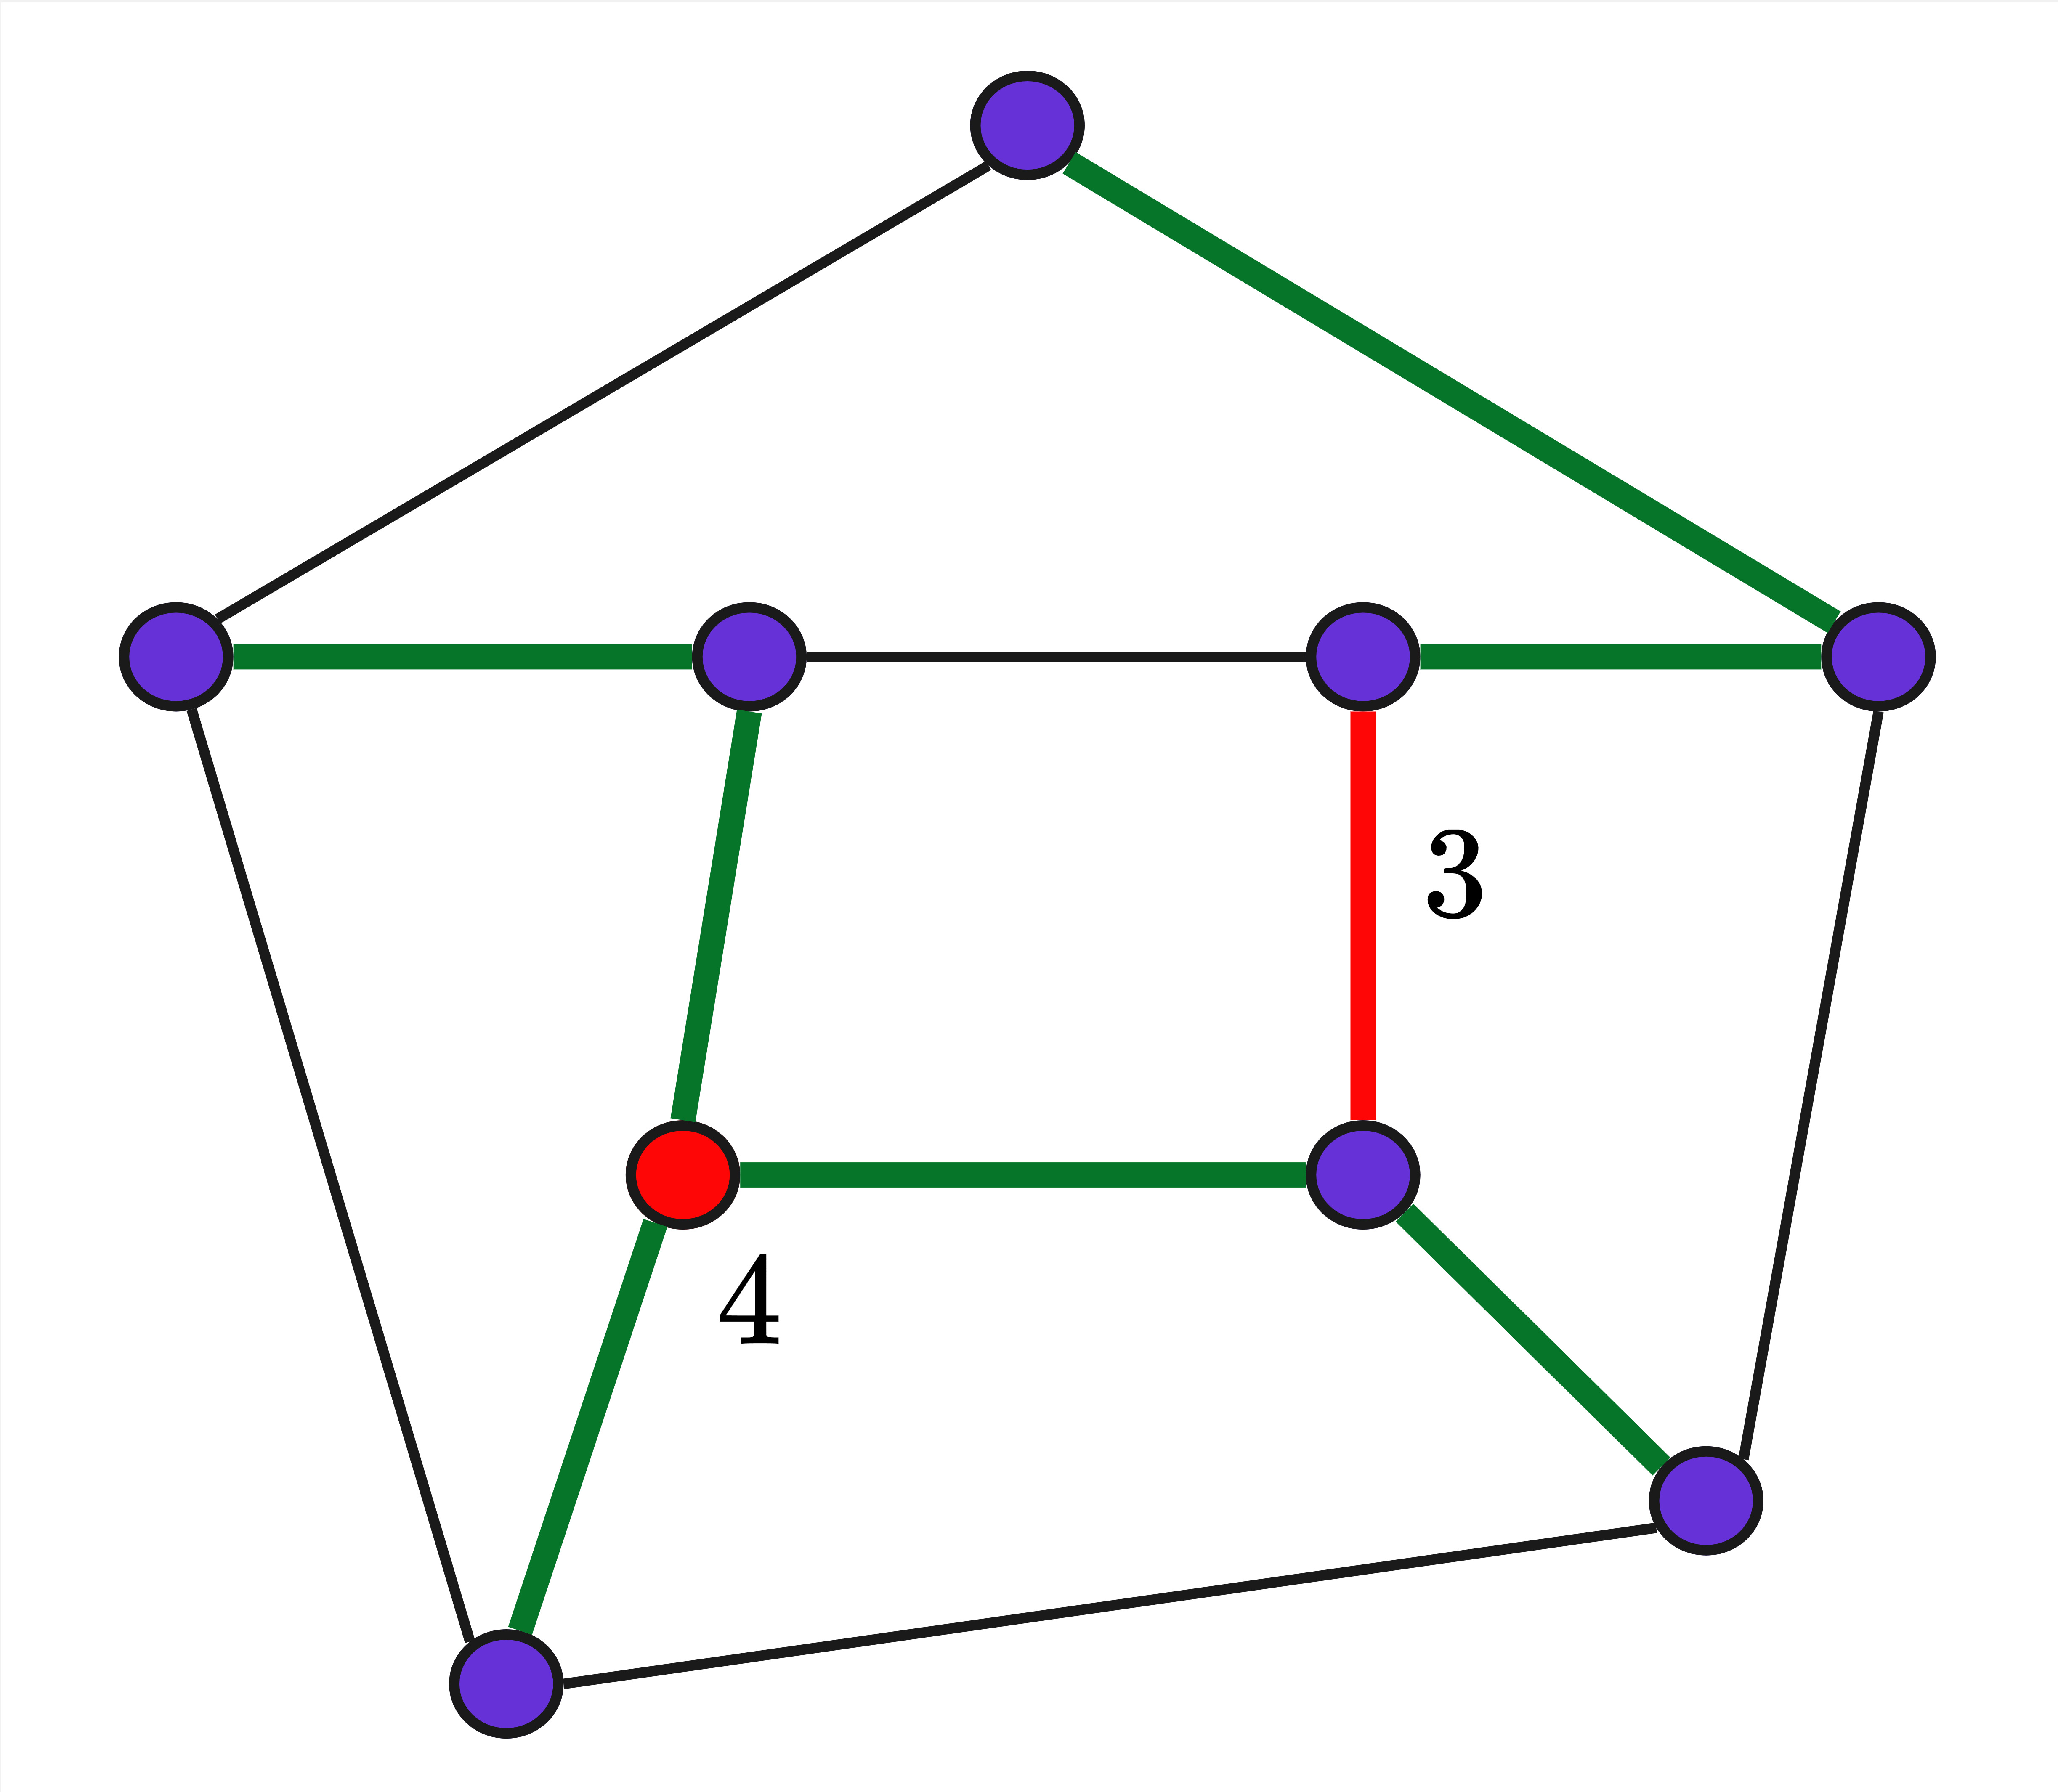
\includegraphics[width=7cm]{images/load_2.jpg}
    \end{minipage}
\end{frame}

\begin{frame}{Última Definição (desta seção)}
    \begin{defi}[Carga Máxima]
        A \emph{\textbf{carga máxima}} de uma floresta geradora maximal $(V, F)$ de um grafo $G$ é o maior valor entre as cargas de seus vértices $v \in V$ e arestas $e \in F$.
    \end{defi}
\end{frame}

\begin{frame}{Passo 2}
    \begin{lema}
        Todo grafo $k$-outerplanar com grau máximo 3 admite uma floresta geradora maximal com carga máxima $\leq 3k$.
    \end{lema}
    \bigbreak\pause
    Procedemos por indução em $k$.
\end{frame}

\begin{frame}{Passo 2\dots}
    \begin{proof}
    Suponha $k = 1$ e seja $R$ o conjunto de arestas da face externa da imersão de $G$:
    \begin{itemize}[-]
        \item Remova $R$; o grafo resultante é acíclico.
        \item Estenda $E \setminus R$ para uma floresta geradora maximal $F$, adicionando o máximo possível de arestas de $R$.
        \item Considere as arestas em $E \setminus F$ e as faces internas que elas formam.
        \item Cada aresta de $G$ delimita no máximo 2 faces internas, e cada vértice $v \in V$ participa de no máximo $\deg(v)$ delas.
    \end{itemize}
    \end{proof}
\end{frame}

\begin{frame}{Exemplo}
    \begin{minipage}{\linewidth}
        \centering
        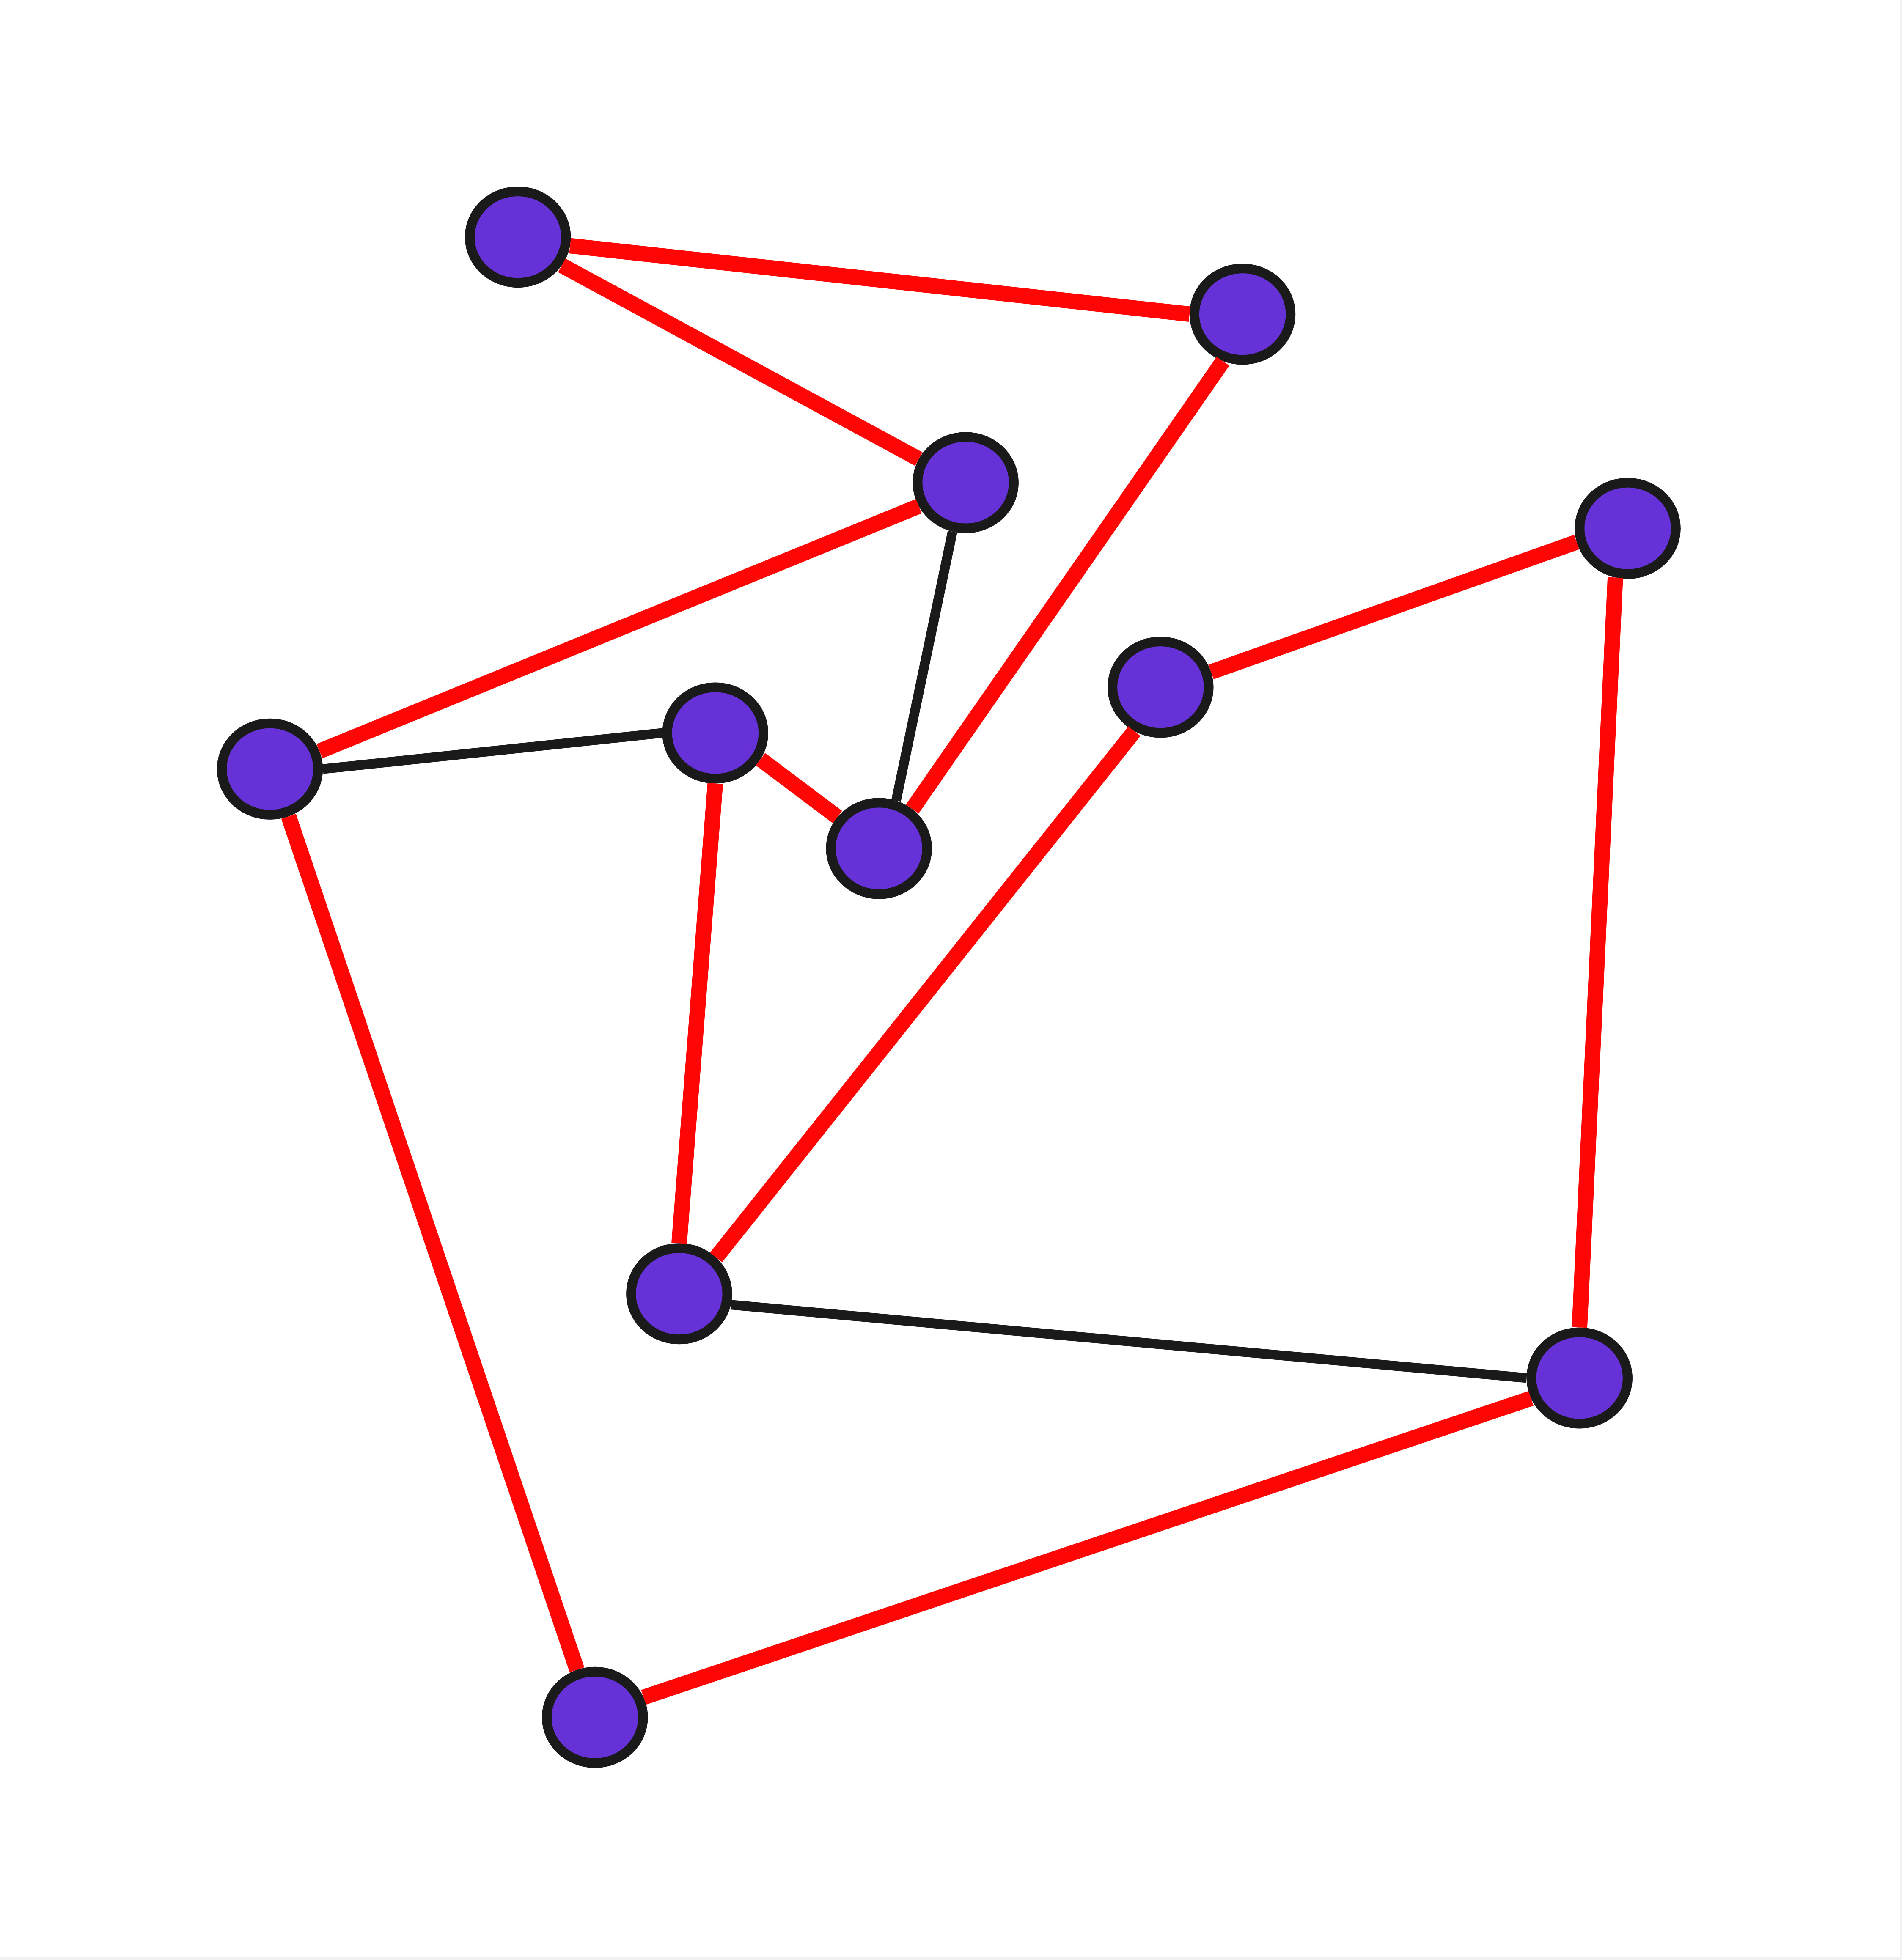
\includegraphics[width=8cm]{images/proof_2_1.jpg}
    \end{minipage}
\end{frame}

\begin{frame}{Exemplo}
    \begin{minipage}{\linewidth}
        \centering
        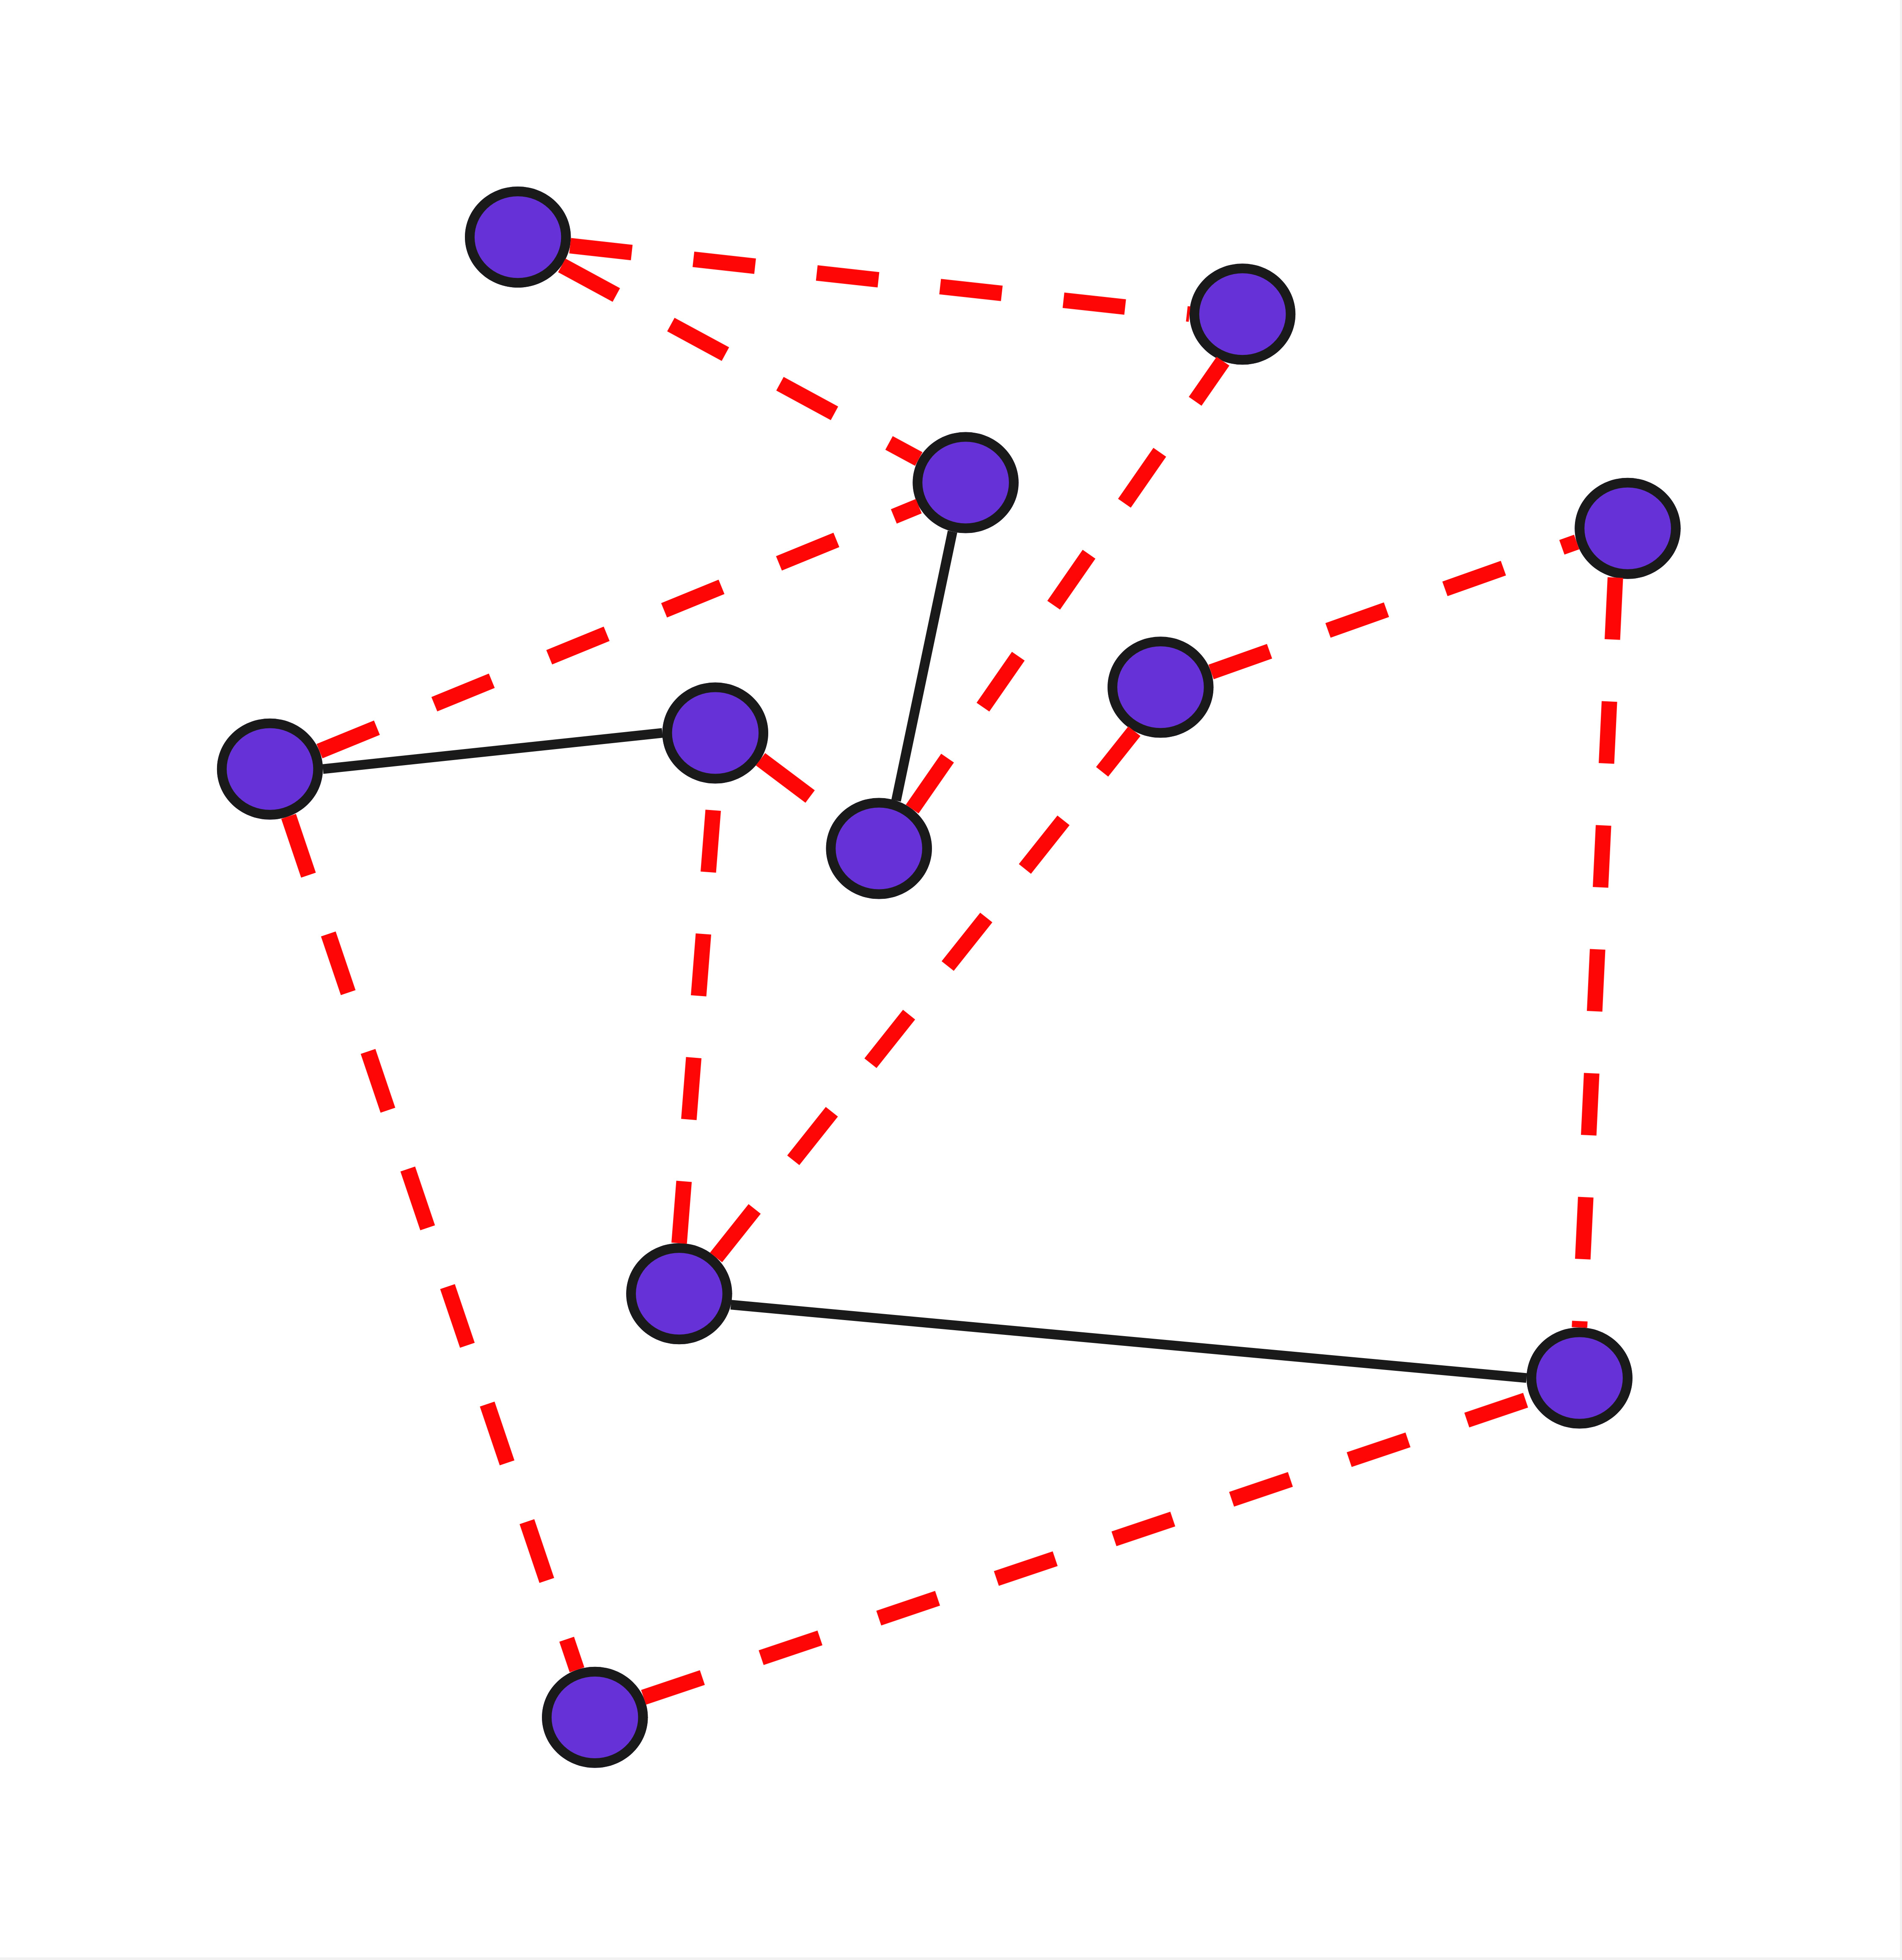
\includegraphics[width=8cm]{images/proof_2_2.jpg}
    \end{minipage}
\end{frame}

\begin{frame}{Exemplo}
    \begin{minipage}{\linewidth}
        \centering
        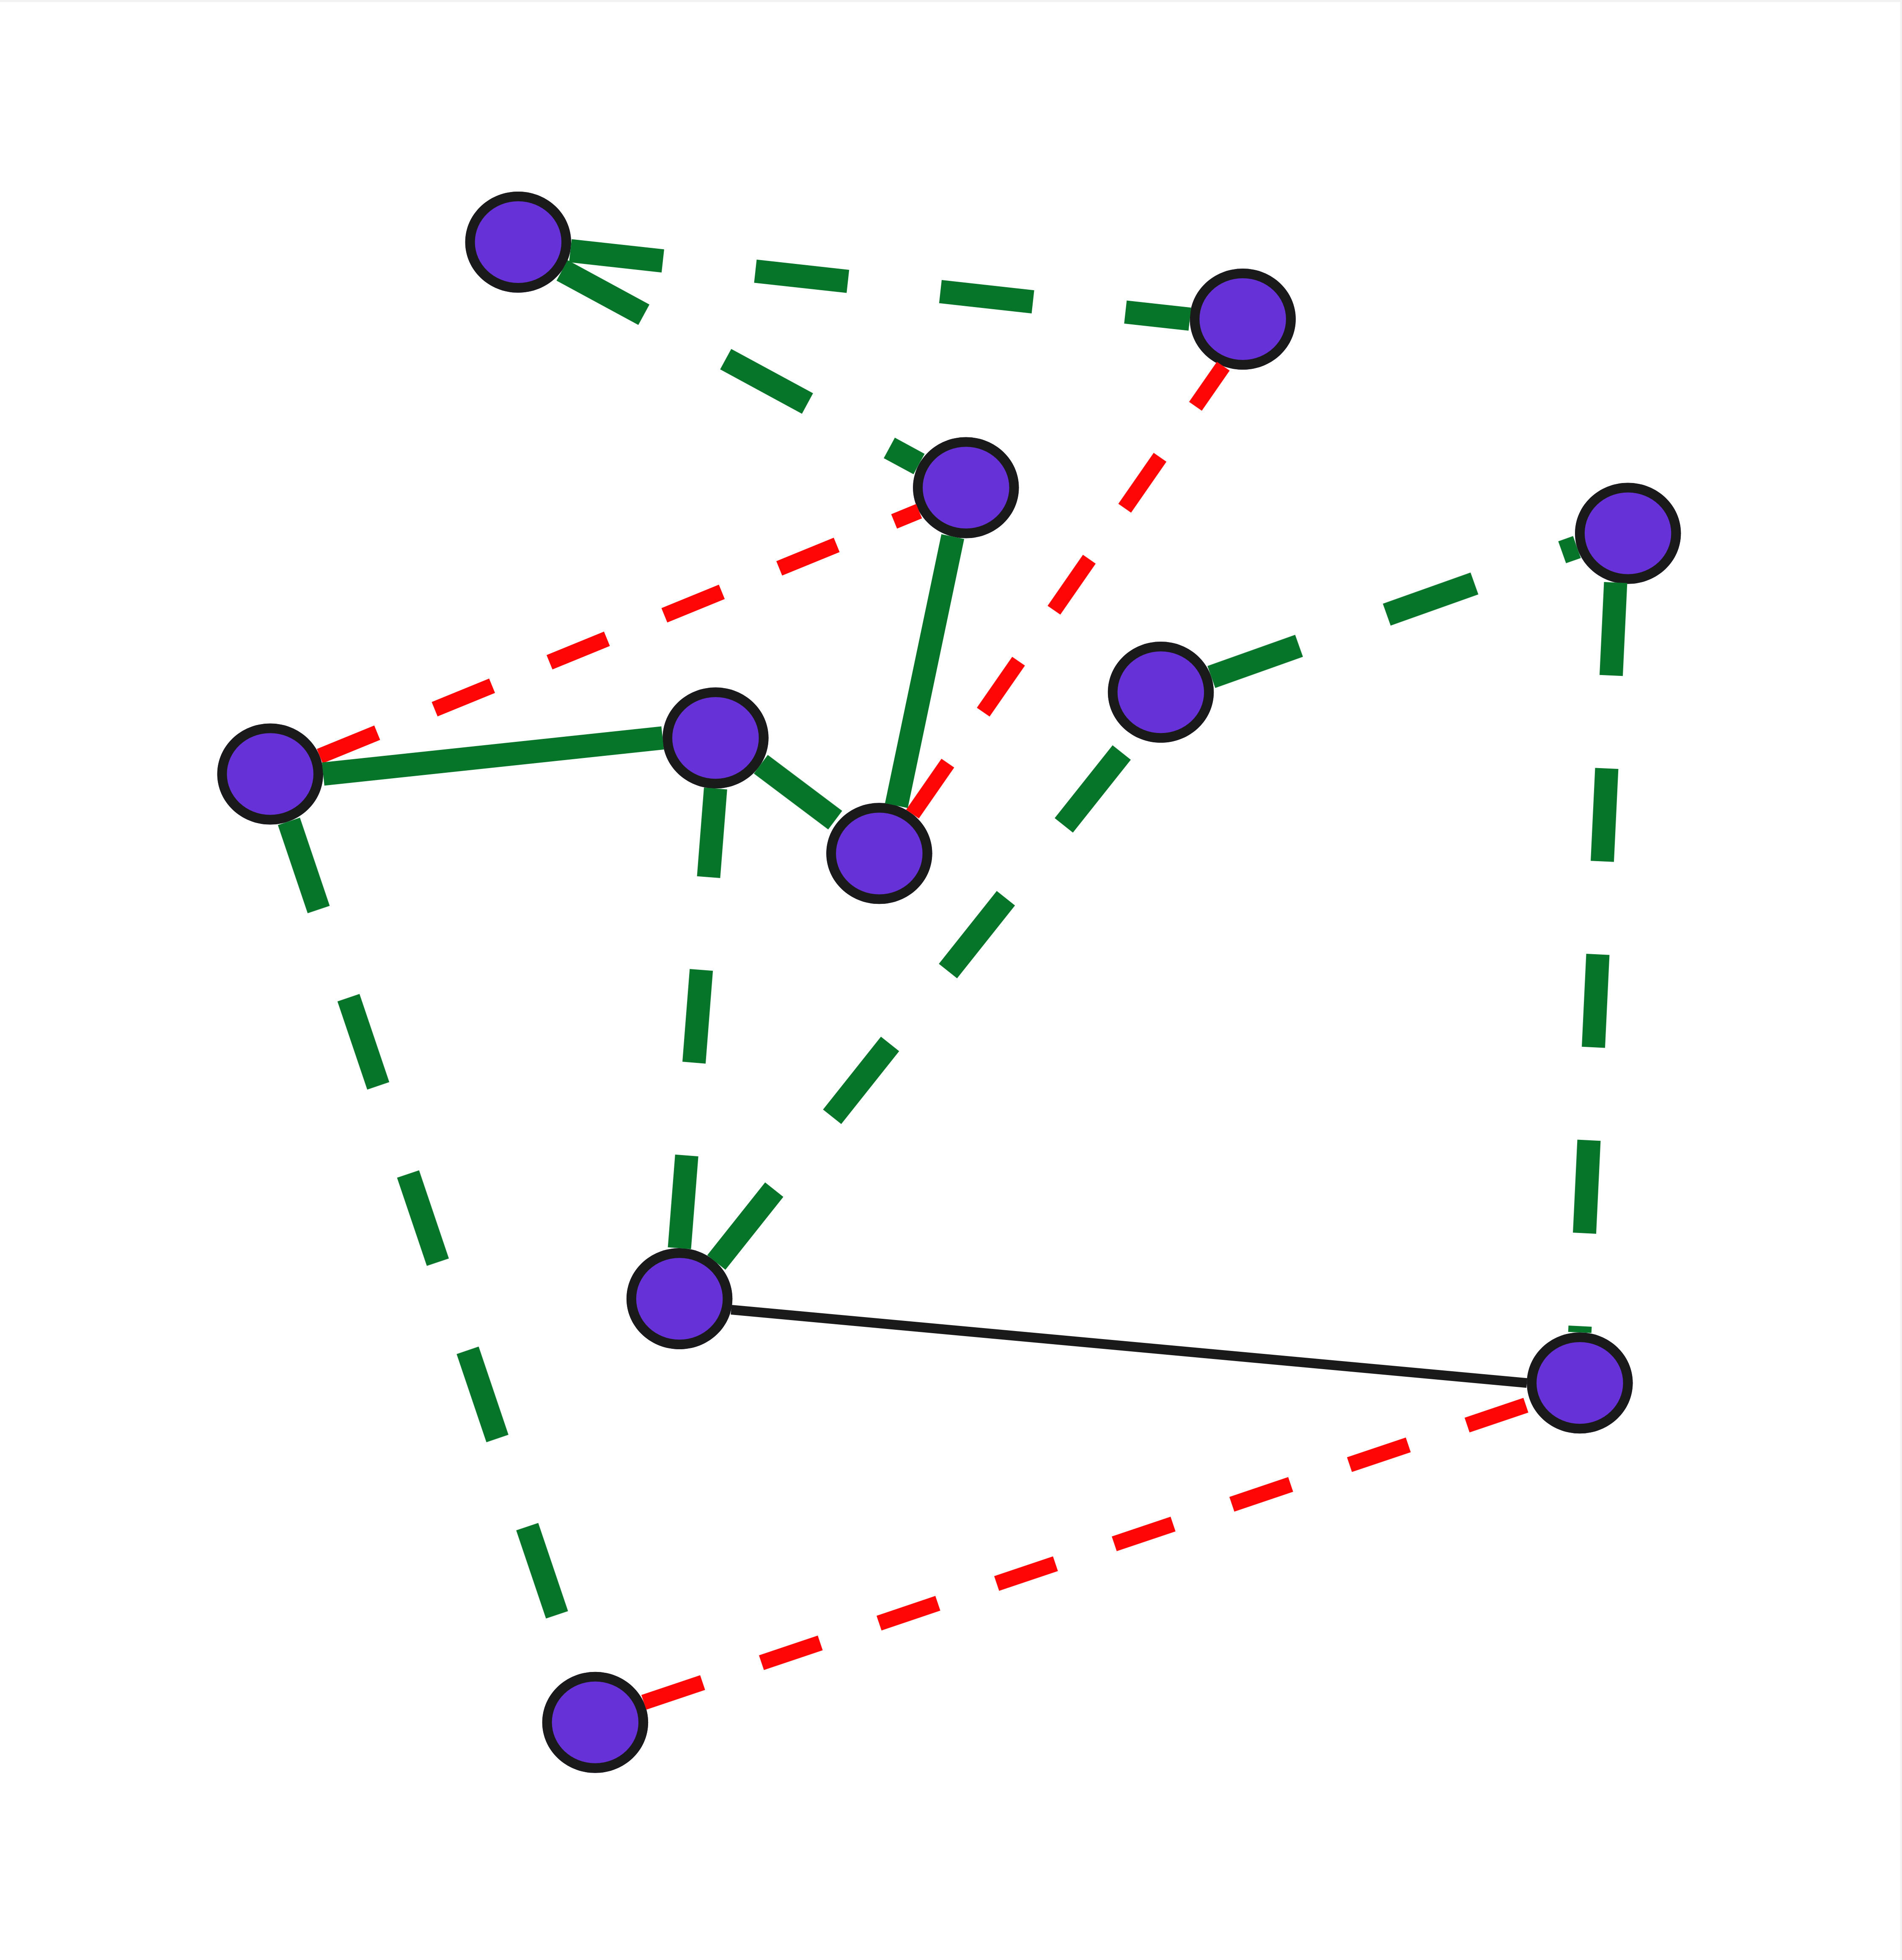
\includegraphics[width=8cm]{images/proof_2_3.jpg}
    \end{minipage}
\end{frame}

\begin{frame}{Passo 2\dots}
    \begin{proof}
        Para $k > 1$, seja $R$ o conjunto de arestas da face externa da imersão de $G$:
        \begin{itemize}[-]
            \item Remova $R$; o grafo restante é, no máximo, $(k - 1)$-outerplanar.
            \item Por indução, existe uma floresta geradora maximal $F^{\prime}$ com carga máxima $\leq 3(k - 1)$.
            \item Estenda $F^{\prime}$ para uma floresta geradora maximal $F$ de $G$, adicionando arestas de $R$.
            \item A carga adicional em qualquer aresta de $F$ é no máximo $2$, e em qualquer vértice, no máximo $3$.
        \end{itemize}
    \end{proof}
\end{frame}

\begin{frame}{Exemplo}
    \begin{minipage}{\linewidth}
        \centering
        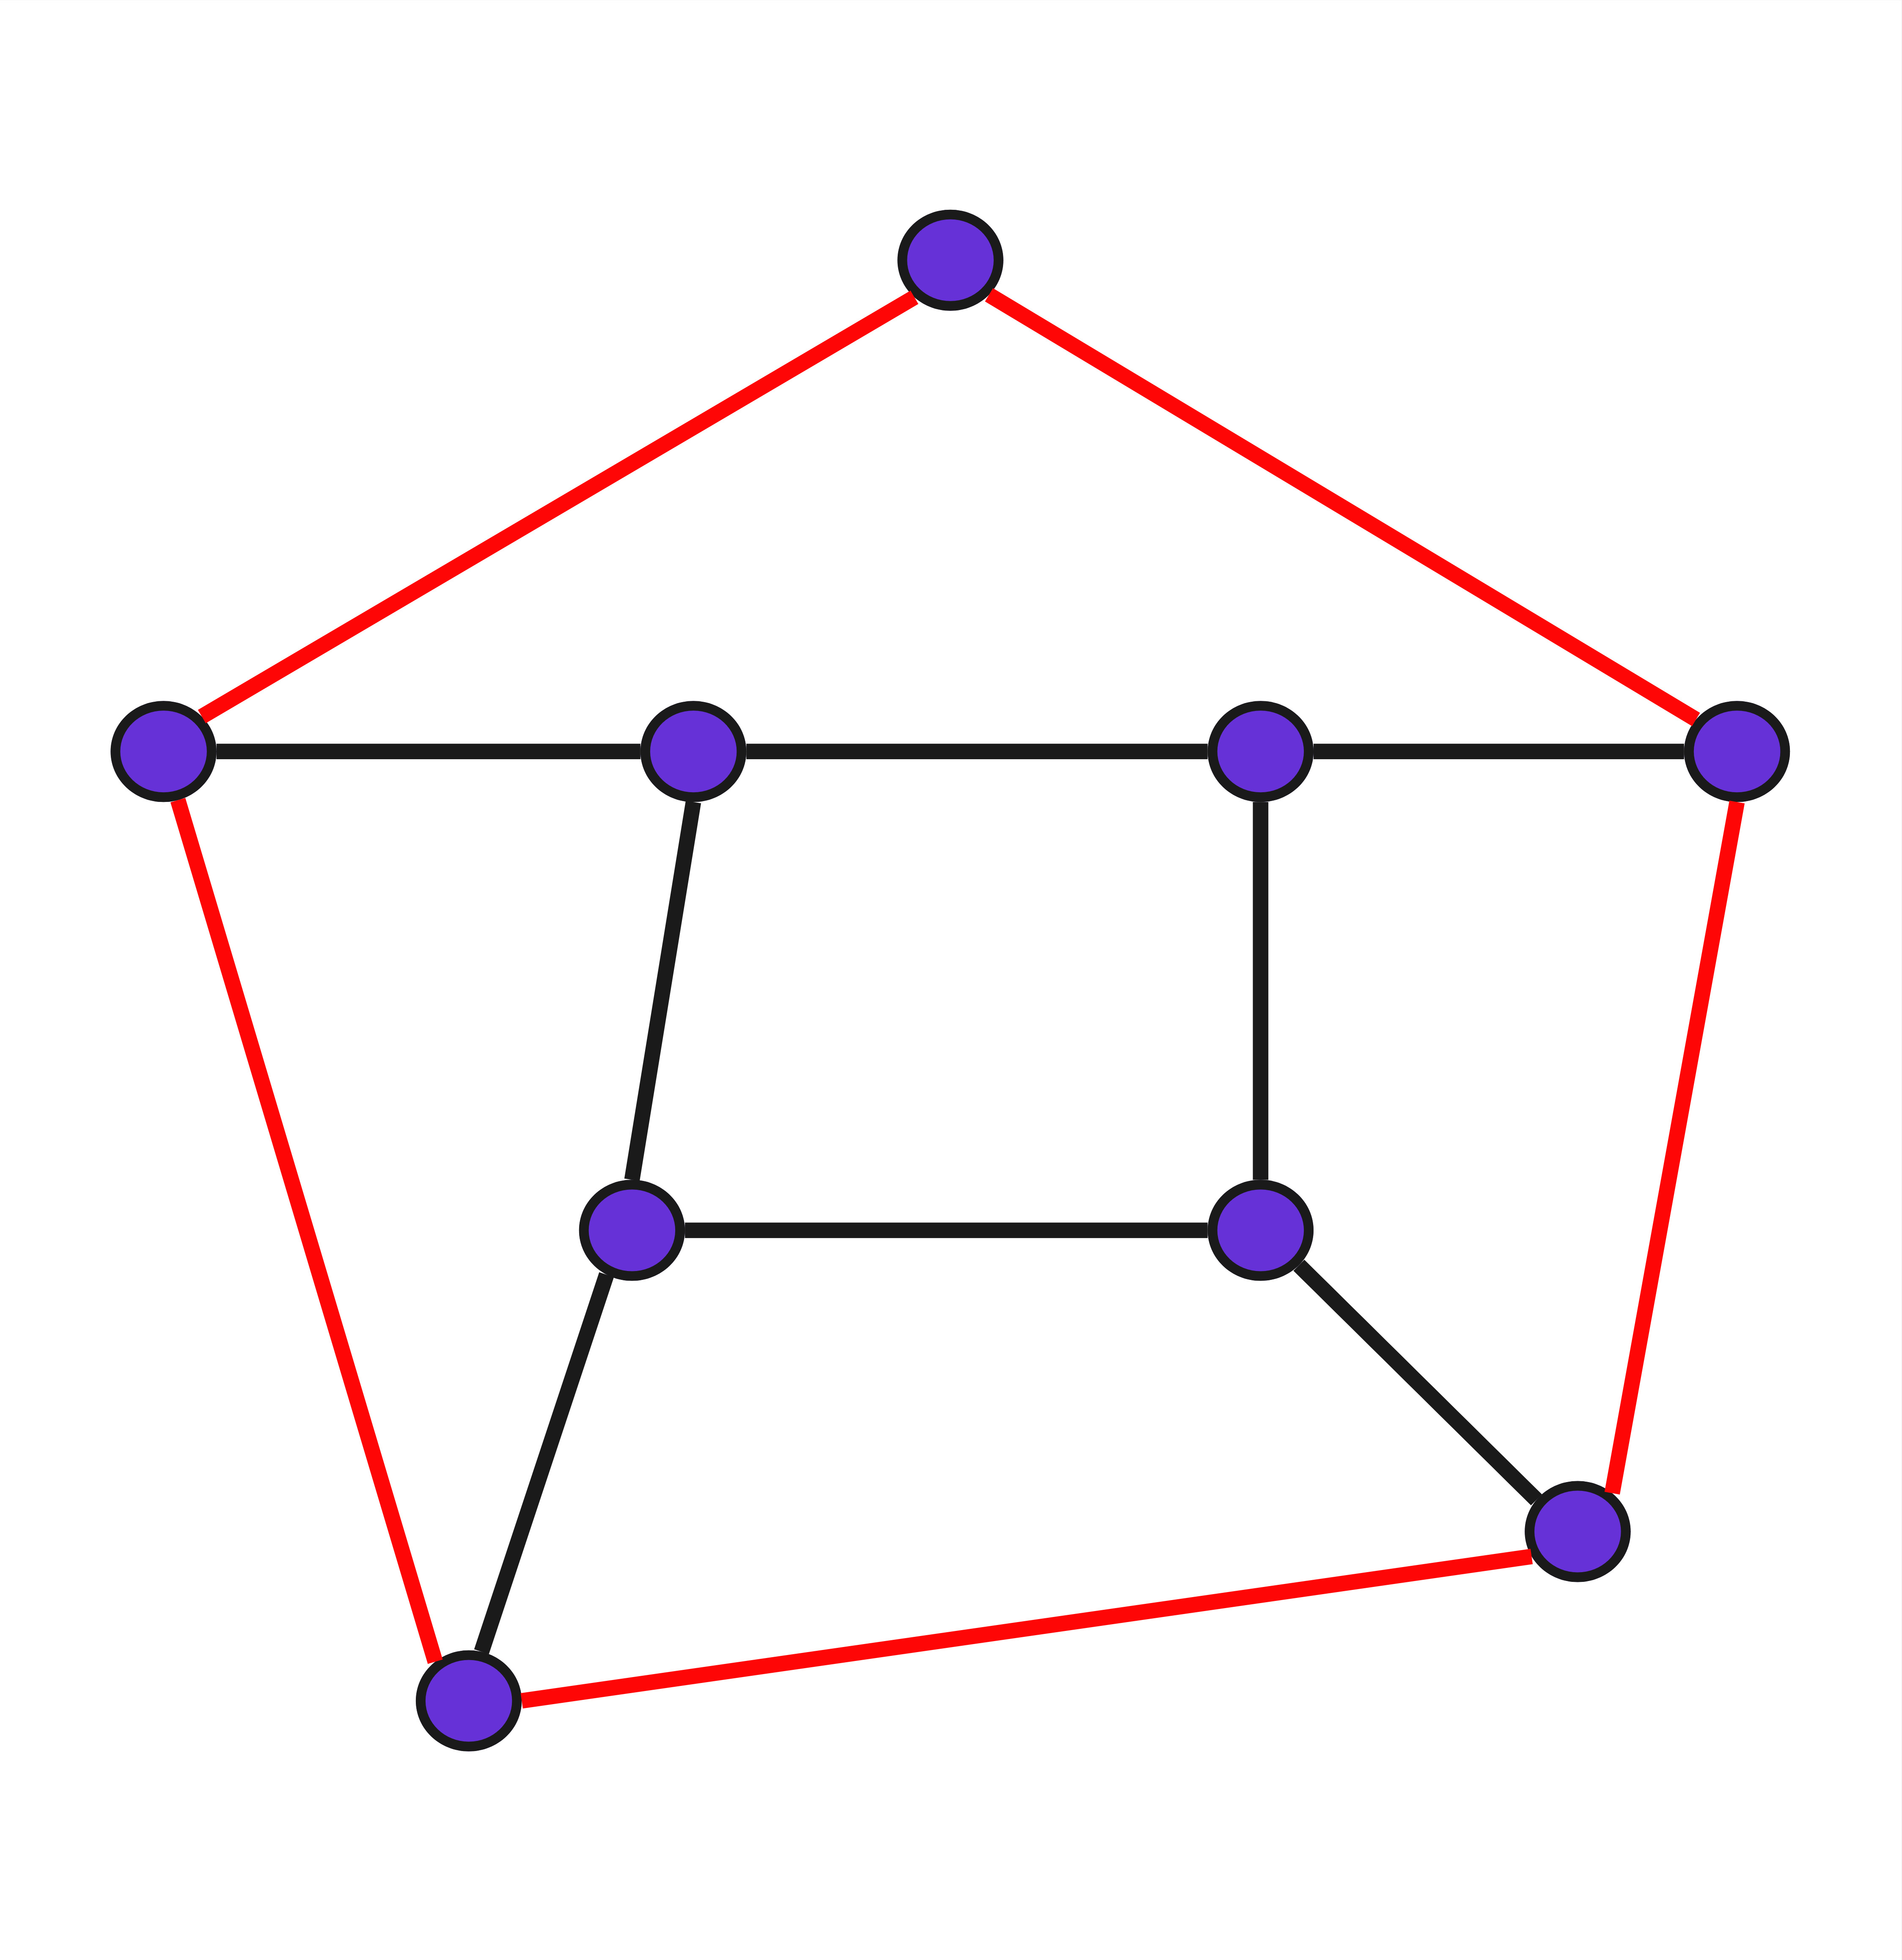
\includegraphics[width=8cm]{images/proof_2_4.jpg}
    \end{minipage}
\end{frame}

\begin{frame}{Exemplo}
    \begin{minipage}{\linewidth}
        \centering
        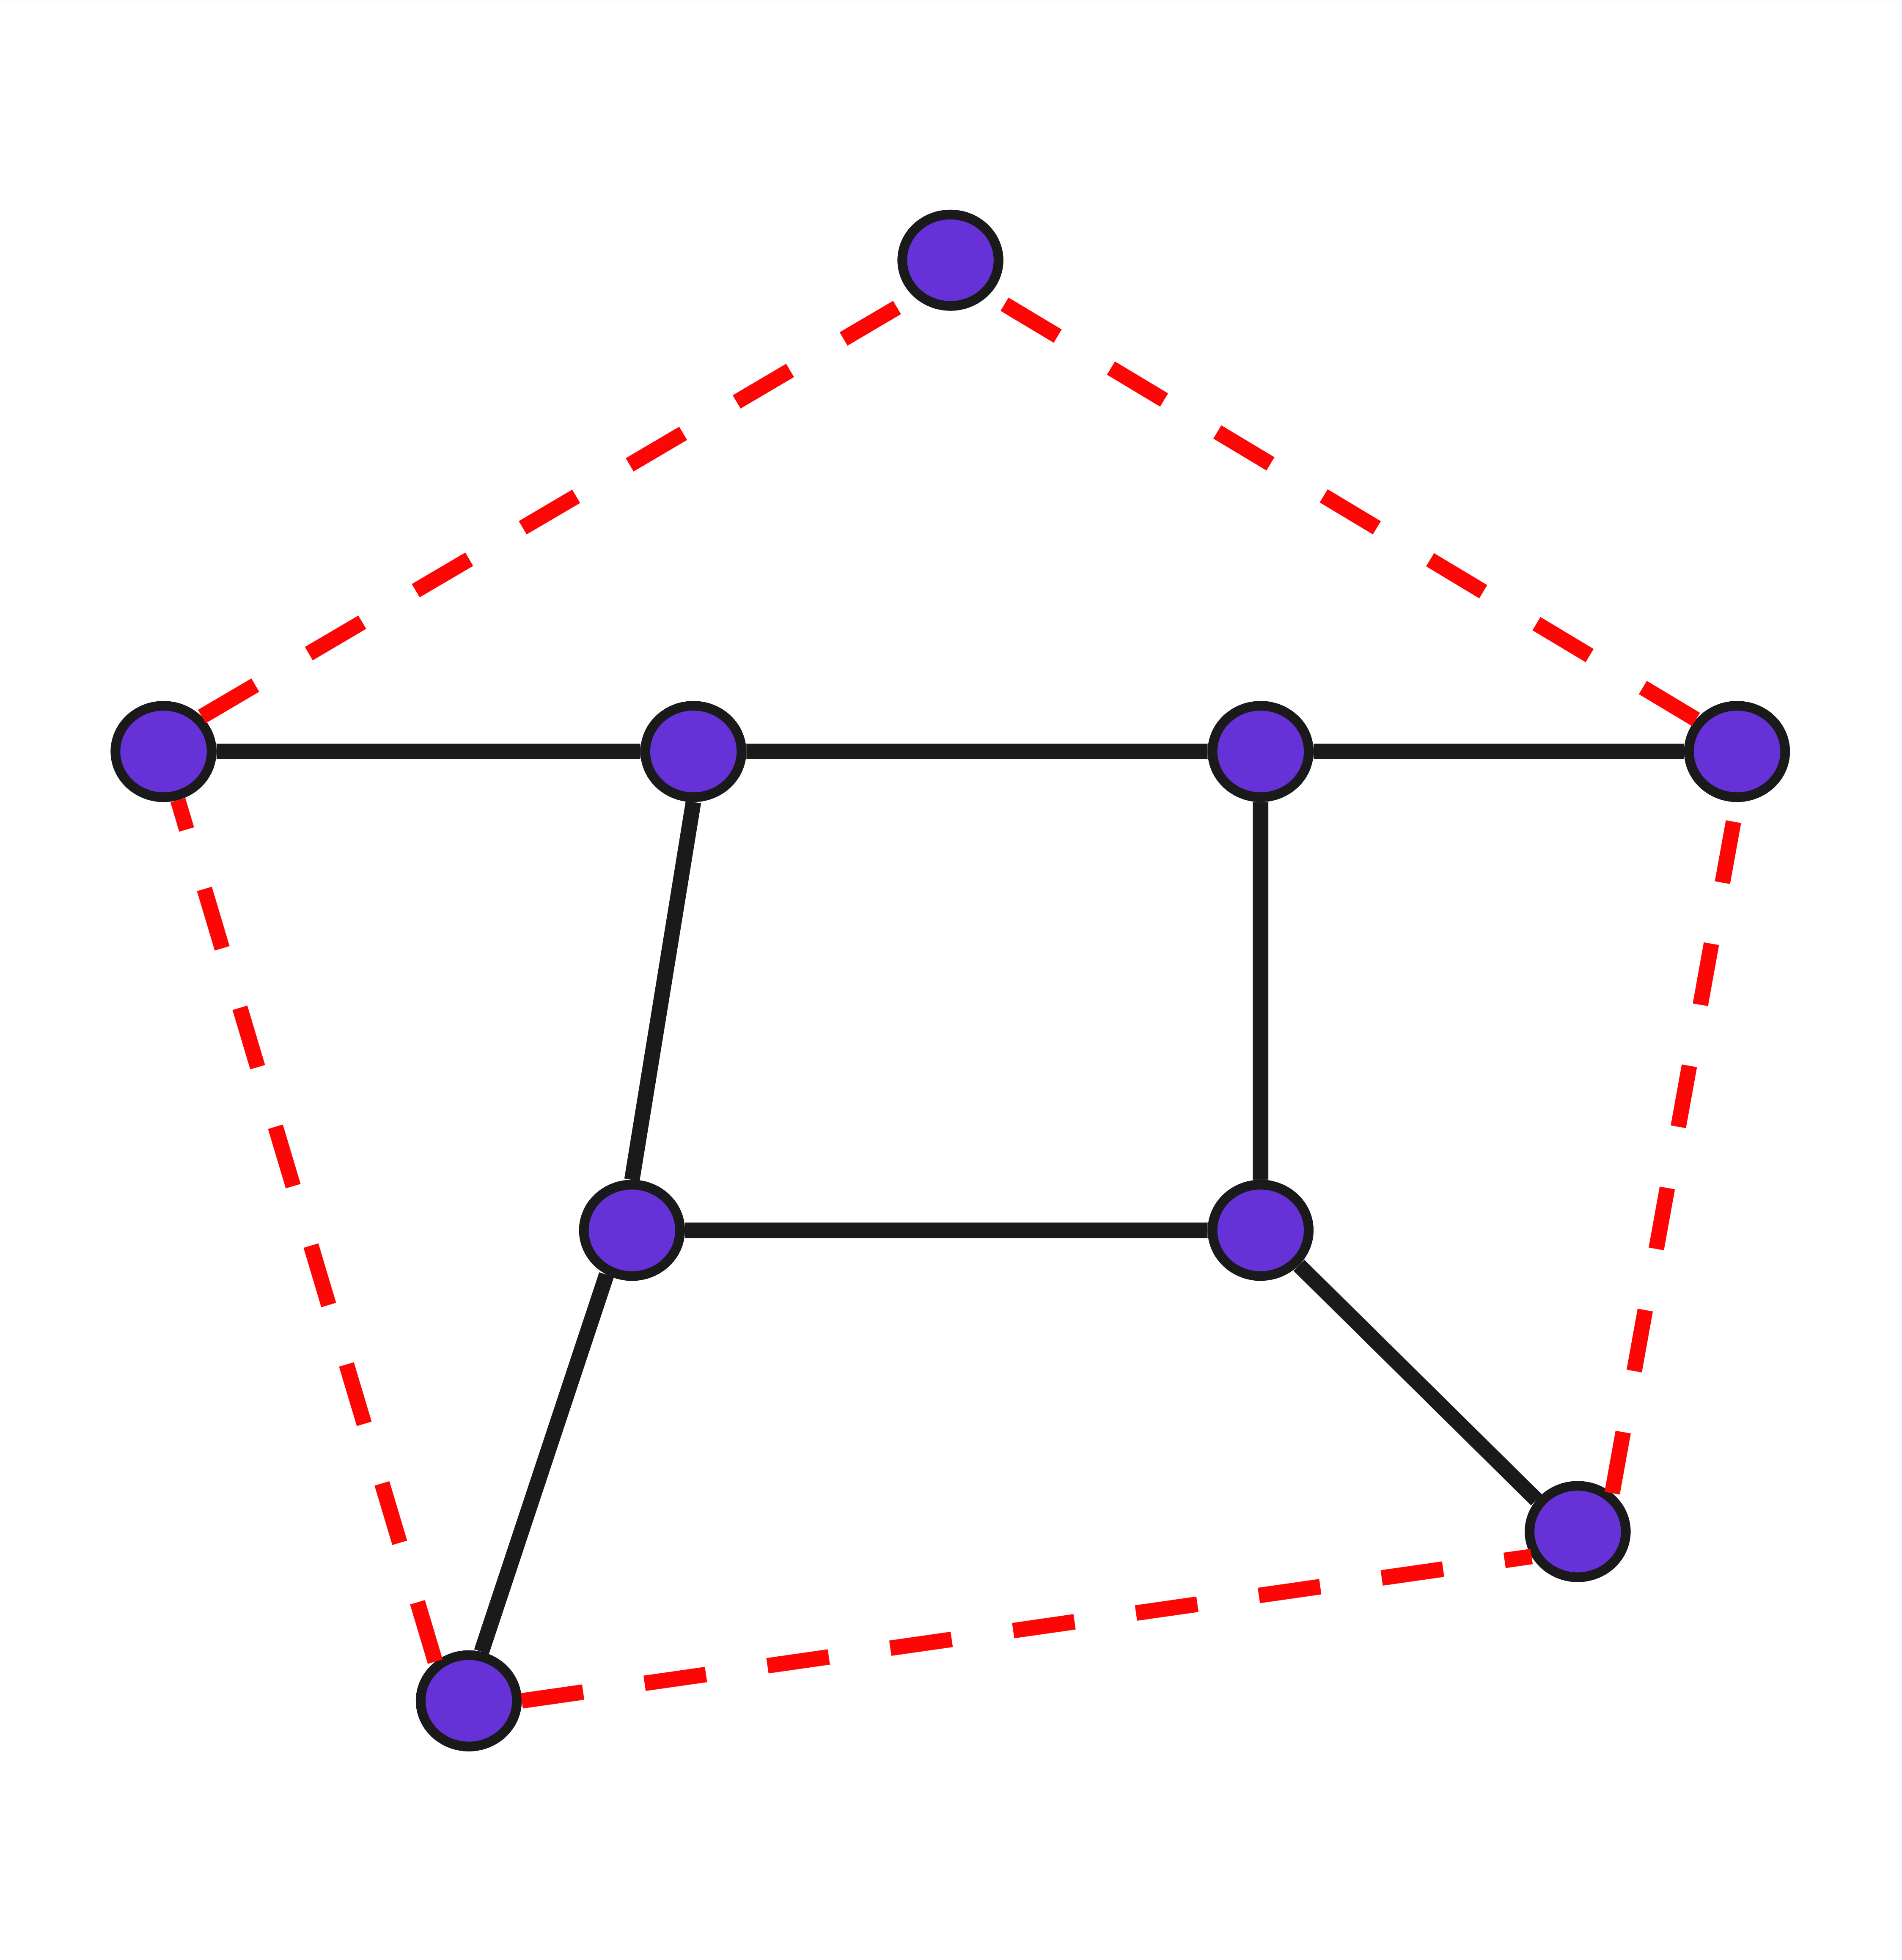
\includegraphics[width=8cm]{images/proof_2_5.jpg}
    \end{minipage}
\end{frame}

\begin{frame}{Exemplo}
    \begin{minipage}{\linewidth}
        \centering
        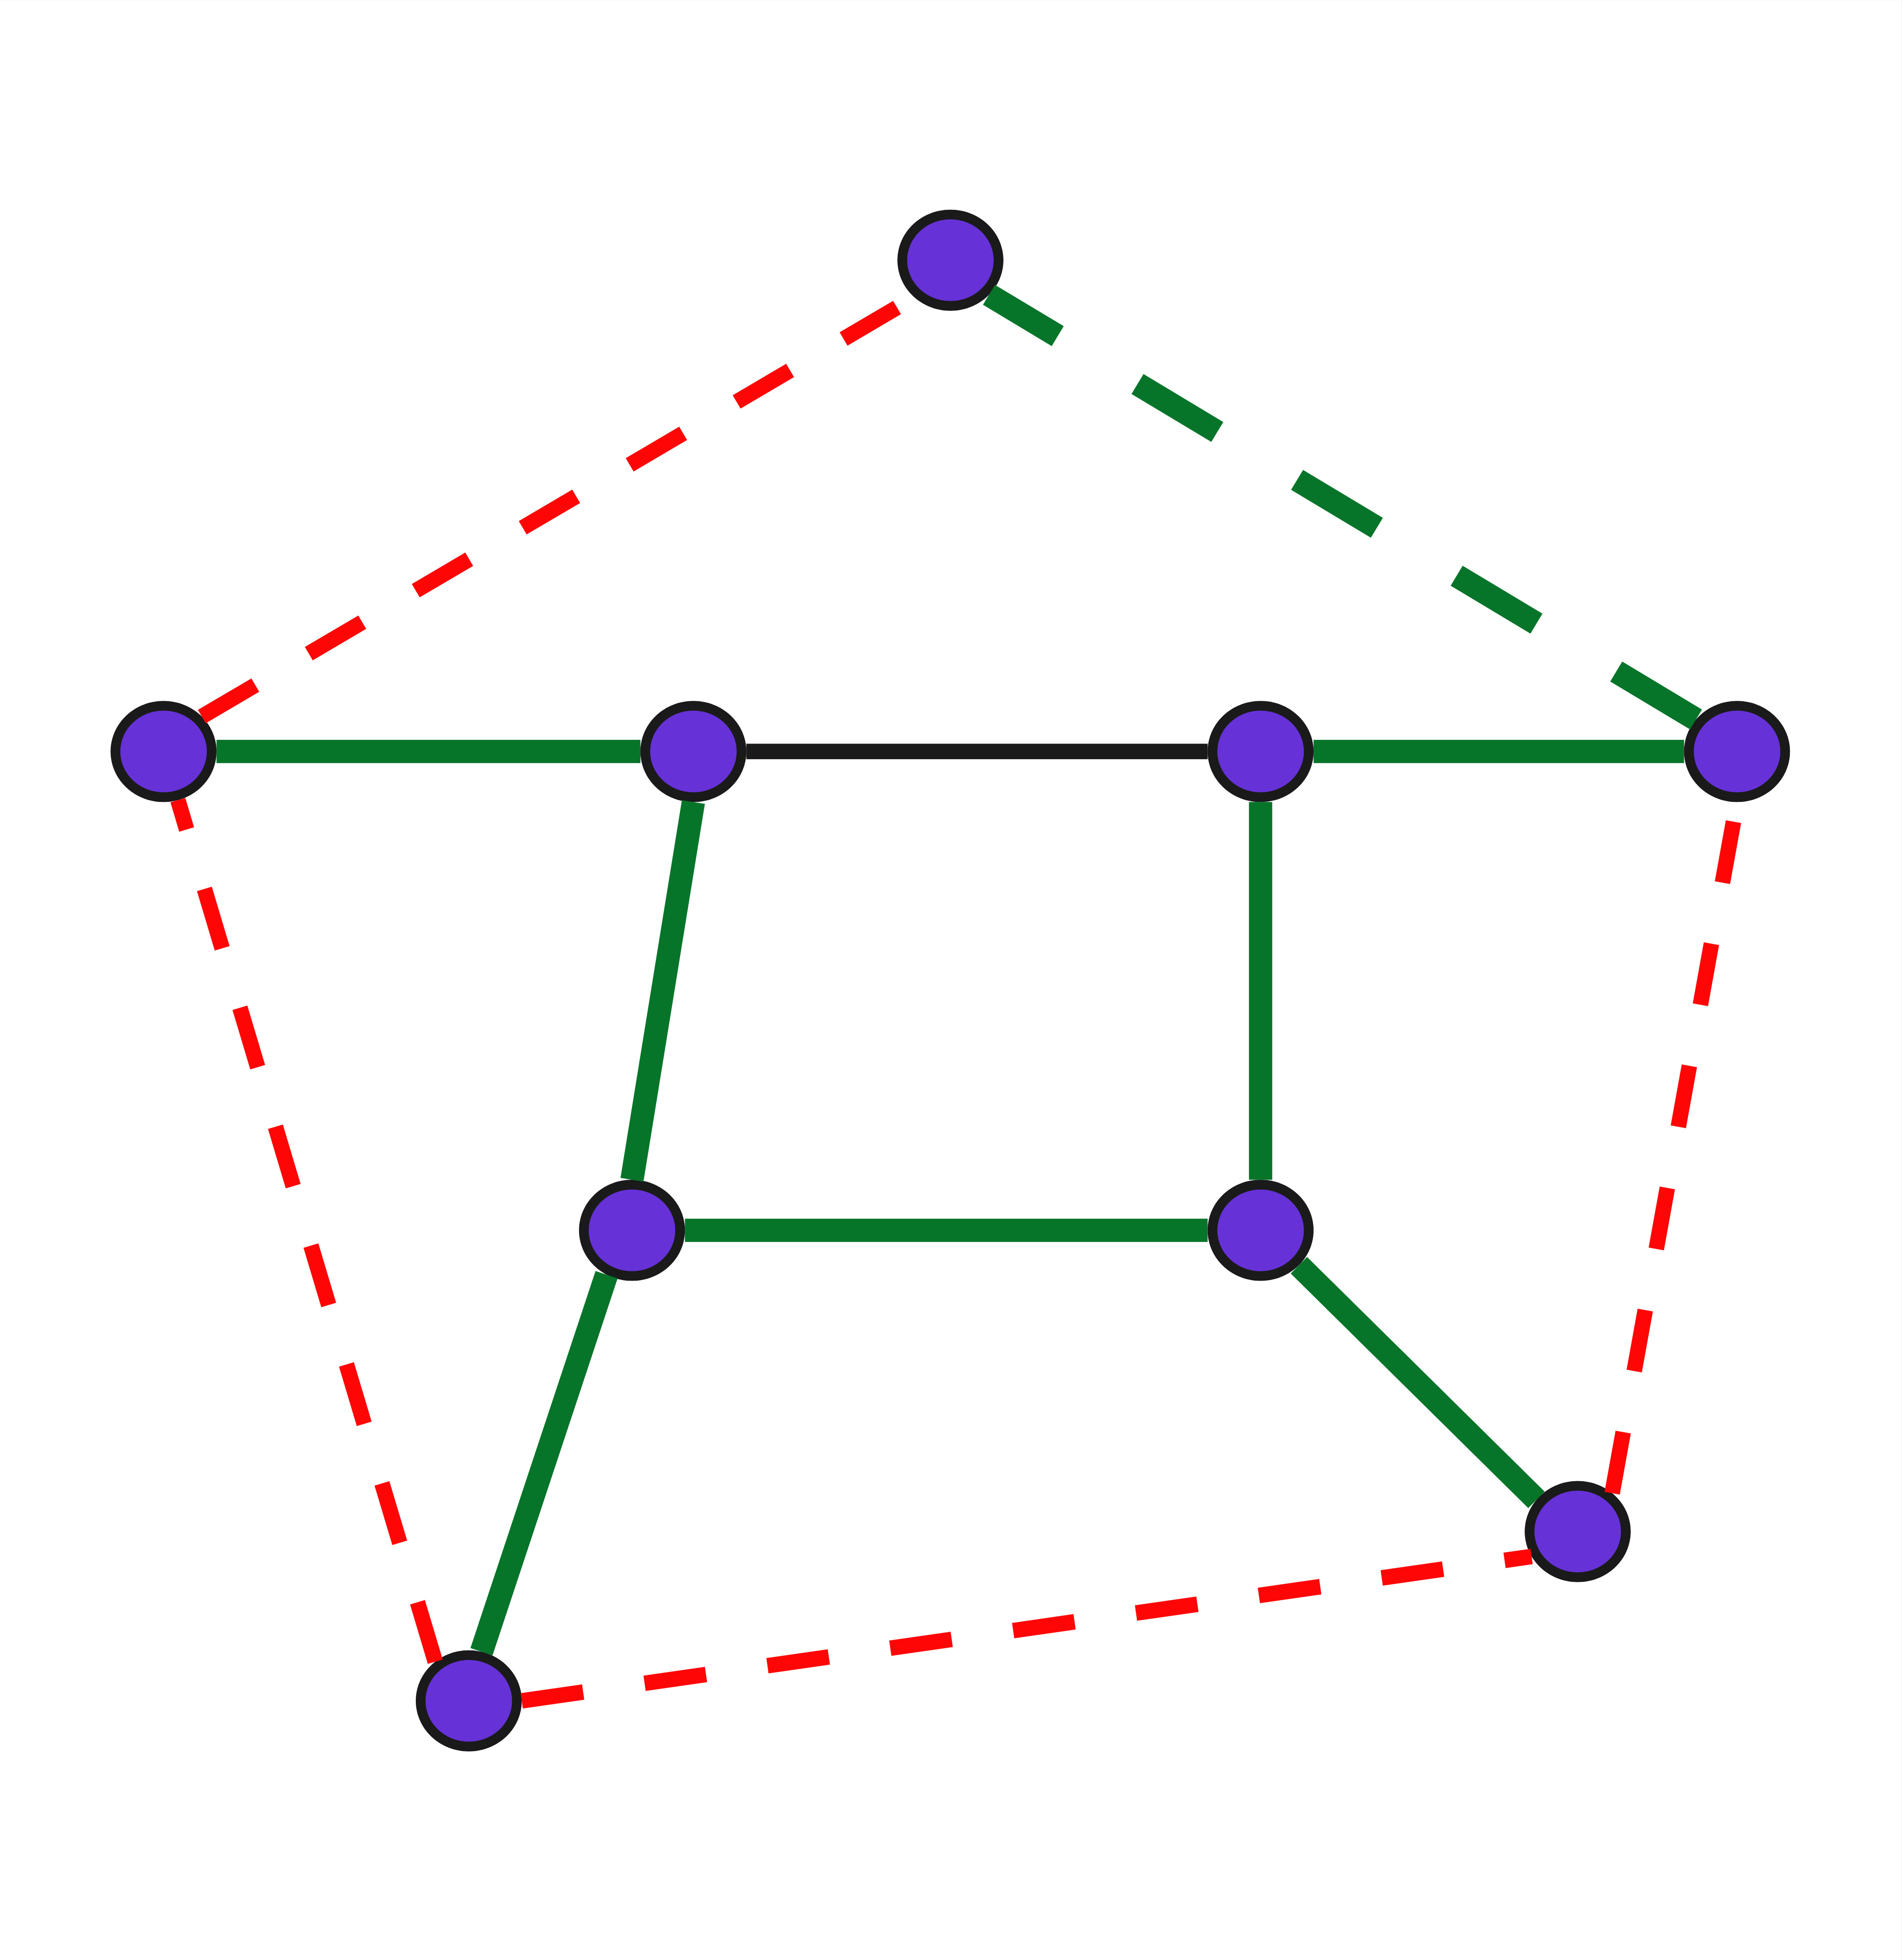
\includegraphics[width=8cm]{images/proof_2_6.jpg}
    \end{minipage}
\end{frame}

\begin{frame}{Passo 3}
    \begin{block}{Lema}
        Se um grafo $G$ de grau máximo 3 admite uma floresta geradora maximal $(V, F)$ com carga máxima $\leq \ell$, então a largura da árvore de $G$ é no máximo $\ell + 1$.
    \end{block}
\end{frame}

\begin{frame}{Passo 3\dots}
    \begin{proof}
        Construa uma decomposição em árvore para a floresta $F$ da seguinte forma:
        \begin{itemize}[-]
            \item Para cada vértice $u \in V$ e cada aresta $e = (v, w) \in F$, crie nós $t_u$ e $t_e$ em $T$.
            \item Iniciamos com $X_u = \{u\}$ e $X_e = \{v, w\}$.
            \item Para cada aresta $e = (u, v) \in E \setminus F$, escolha arbitrariamente um de seus extremos, digamos $u$.
            \item Para cada vértice $w \neq v$ no ciclo fundamental de $e$, adicione $u$ a $X_w$.
            \item Para cada aresta $e^\prime \in F$ no ciclo fundamental de $e$, adicione $u$ a $X_{e^\prime}$.
        \end{itemize}
        \phantom{\qedhere}
    \end{proof}
\end{frame}

\begin{frame}{Passo 3\dots}
    \begin{proof}
        Note que $(T, \{X_t\}_{t \in V(T)})$ é uma decomposição em árvore de $G$:
        \bigbreak

        \begin{itemize}
            \item \textbf{Propriedade 1:} Satisfeita trivialmente.
            \item \textbf{Propriedade 2:} Para $e = (u,v) \in E \setminus F$, $u$ foi adicionado a algum $X_{(w,v)}$ no ciclo fundamental de $e$, garantindo que $u$ e $v$ coexistem em um mesmo conjunto.
            \item \textbf{Propriedade 3:} Sempre que um vértice $v$ foi adicionado a subconjuntos, isso ocorreu ao longo de um caminho da árvore, mantendo a propriedade de conectividade.
        \end{itemize}
        \pause\bigbreak

        Cada conjunto $X_u$ ou $X_e$ recebeu no máximo tantos vértices quanto a carga de $u \in V$ ou $e \in F$, respectivamente. Como os conjuntos iniciais tinham no máximo 2 vértices, o tamanho final é no máximo $\ell + 2$.
        \alt<6>{\qedhere}{\phantom\qedhere}
    \end{proof}
\end{frame}

\begin{frame}{Exemplo}
    \begin{minipage}{\linewidth}
        \centering
        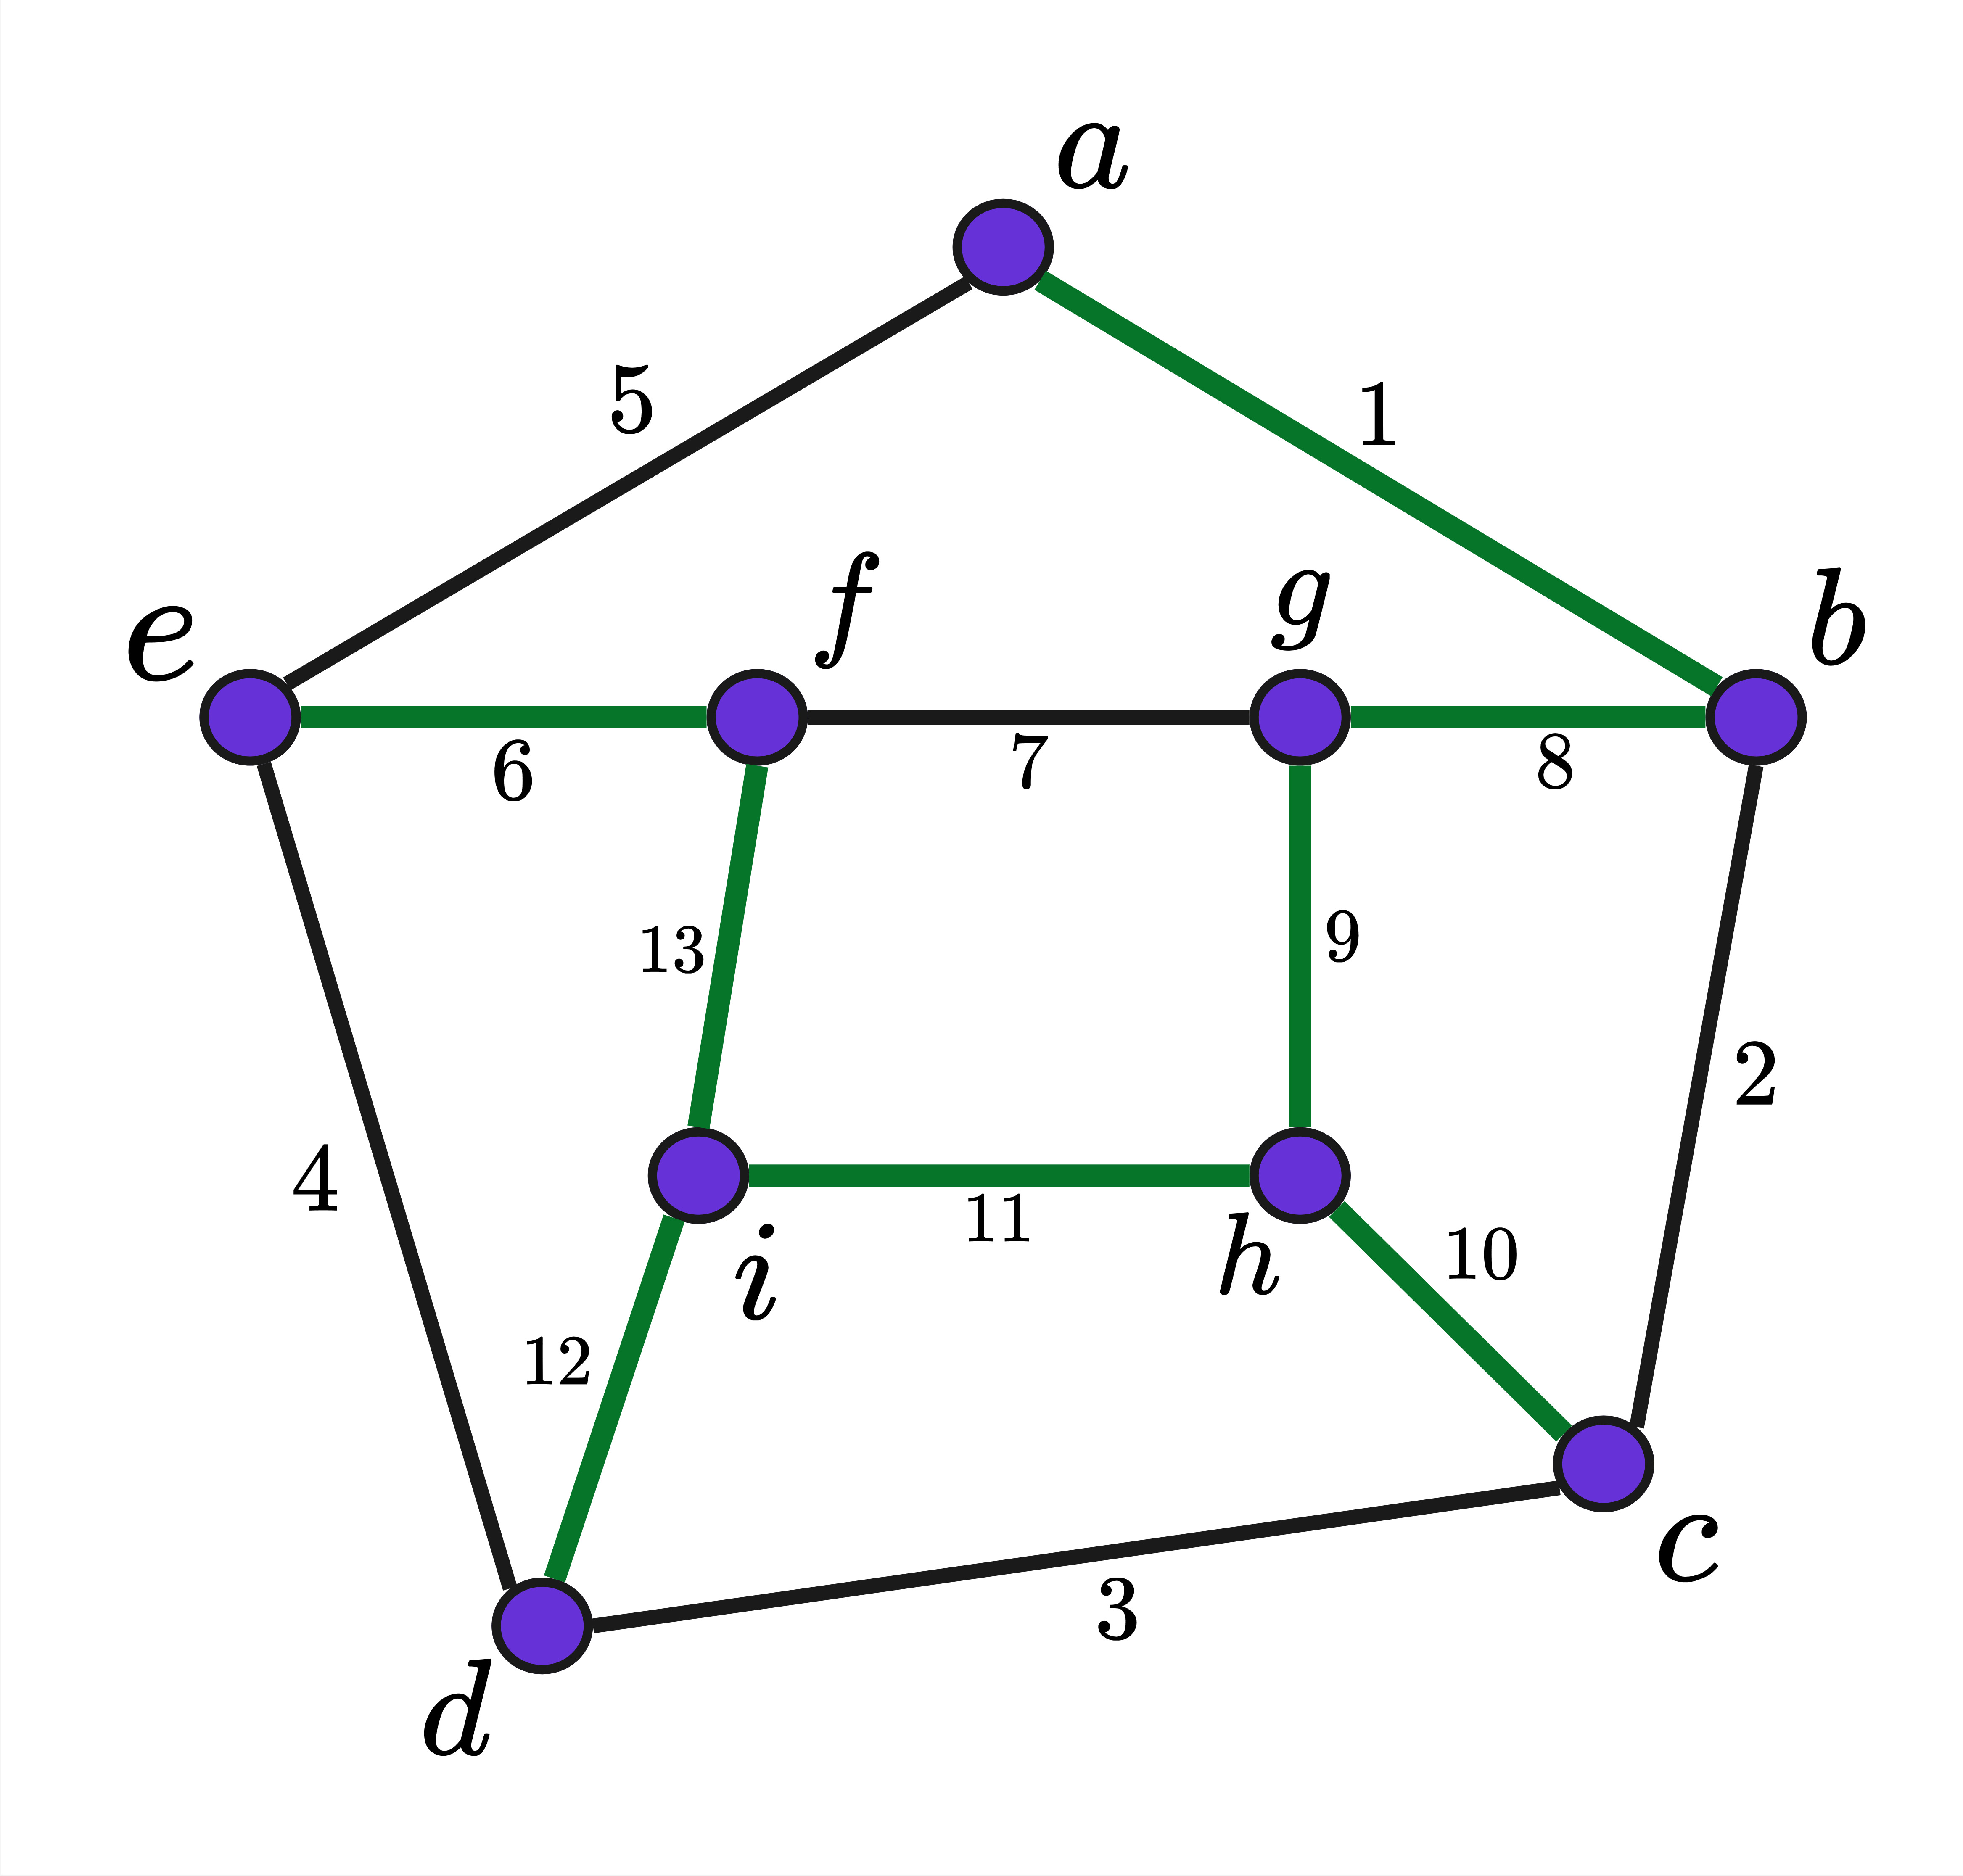
\includegraphics[width=8cm]{images/proof_3.jpg}
    \end{minipage}
\end{frame}

\begin{frame}{Lema Principal}
    \begin{lema}[1]
        \label{lema:1}
        Há um algoritmo para CI em grafos $k$-outerplanar que executa em tempo $2^{O(k)} \cdot n$.
    \end{lema}
\end{frame}
